\documentclass{article}
%encoding
%--------------------------------------
\usepackage[utf8]{inputenc}
\usepackage[T1]{fontenc}
%--------------------------------------
 
%German-specific commands
%--------------------------------------
\usepackage[ngerman]{babel}
\usepackage{csquotes}
%--------------------------------------

%Pictures
%--------------------------------------
\usepackage{graphicx}
\graphicspath{ {./Pictures/} }
\usepackage{tikz}
\usepackage{subcaption}
\usepackage{float}
\usepackage{wrapfig}
%--------------------------------------

%math
%--------------------------------------
\usepackage{amsmath}
\usepackage{amssymb}
\usepackage{amsfonts}
%--------------------------------------

%Frames
%--------------------------------------
\usepackage{framed}

%Colors
%--------------------------------------
\usepackage{xcolor}
\definecolor{blue-violet}{rgb}{0.54, 0.17, 0.89}
\definecolor{codegreen}{rgb}{0,0.6,0}
\definecolor{codegray}{rgb}{0.5,0.5,0.5}
\definecolor{codepurple}{rgb}{0.58,0,0.82}
\definecolor{backcolour}{rgb}{0.95,0.95,0.92}

%--------------------------------------
\usepackage{multicol}
\usepackage[shortlabels]{enumitem}

%Aufgaben
%--------------------------------------
\newtheorem{aufgabe}{Aufgabe}[section]
\newtheorem{definition}{Definition}[section]
\newtheorem{beispiel}{Beispiel}[section]
%--------------------------------------

%Listings
%--------------------------------------
\usepackage{ulem}
\usepackage{listings}
 
\lstdefinestyle{mystyle}{
    backgroundcolor=\color{backcolour},   
    commentstyle=\color{codegreen},
    keywordstyle=\color{magenta},
    numberstyle=\tiny\color{codegray},
    stringstyle=\color{codepurple},
    basicstyle=\ttfamily\footnotesize,
    breakatwhitespace=false,         
    breaklines=true,                 
    captionpos=b,                    
    keepspaces=true,                 
    numbers=left,                    
    numbersep=5pt,                  
    showspaces=false,                
    showstringspaces=false,
    showtabs=false,                  
    tabsize=2,
}
 
\lstset{style=mystyle,moredelim=[is][\sout]{|}{|}}
%--------------------------------------


\title{Die Breitensuche -- eine Einführung für Schüler der Gymnasialstufe}
\author{eglimu, amaximov}
\date{November 2019}

\begin{document}

\maketitle

\tableofcontents

\section{Einführung}
\begin{figure}[h]
    \centering
    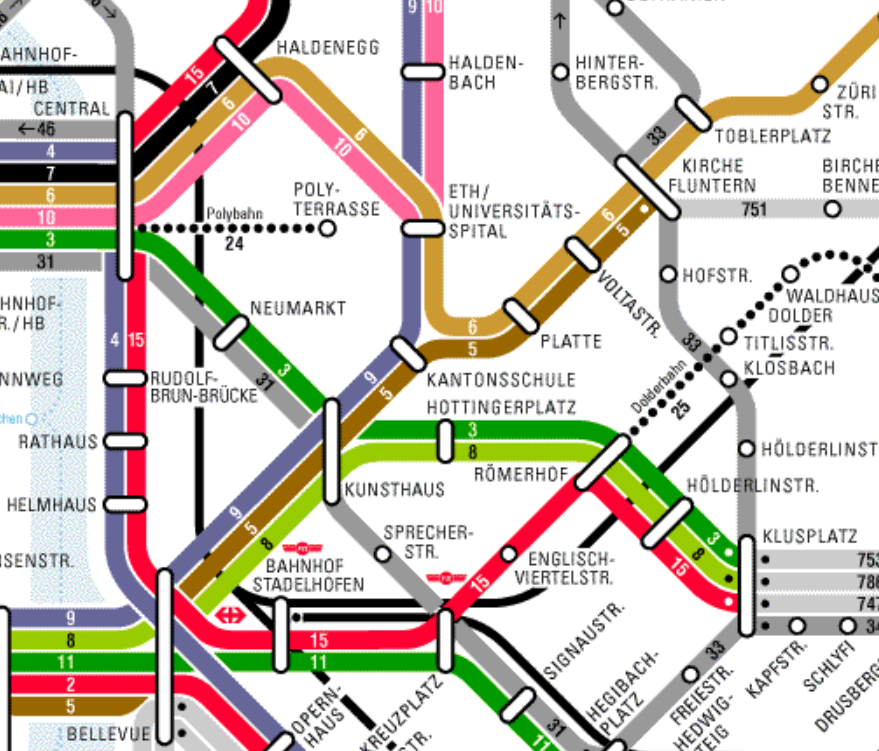
\includegraphics[width=\linewidth]{Pictures/Tram1.PNG}
    \caption{Ein Ausschnitt der Tram- und Buslinien in Zürich}
\end{figure}

Alice steht nach der Schule an der Haltestelle ''Kantonsschule'' in Zürich und möchte einen ganz bestimmten Kugelschreiber einkaufen gehen. Ihr Ziel ist es möglichst wenige Zwischenhaltestellen zu besuchen, bevor sie eine erreicht, in deren Nähe ein Laden mit genau diesem Kugelschreiber im Sortiment steht. Sie beginnt also zu überlegen: ''Die benachbarten Haltestellen sind\\ ''ETH/Universitätsspital'', ''Platte'' und ''Kunsthaus'', aber bei keiner dieser Stationen finde ich meinen Kugelschreiber. Nun kann ich von diesen drei Haltestellen wiederum für alle Benachbarten überlegen ob es dort den Kugelschreiber gibt, denn das sind genau jene Stationen, die ich mit nur einem Zwischenstopp erreichen kann.'' Auf diese Art überlegt Alice weiter, bis sie eine Haltestelle findet, in deren Nähe der Kugelschreiber verkauft wird. \\

Das Problem der Suche nach dem Kugelschreiber können wir als Graphenproblem formalisieren, indem wir für jede Haltestelle einen Knoten zeichnen und jeweils die Benachbarten mit einer Kante verbinden. Alice beginnt also bei ihrem Startknoten ''Kantonsschule'' und durchläuft dann die restliche Knoten, aufsteigend geordnet nach dem Abstand zu diesem Startknoten. Erinnere dich, dass wir den Abstand von zwei Knoten in einem Graphen definiert haben als die Anzahl Kanten des kürzesten Pfades vom ersten Knoten zum zweiten. Das von Alice durchgeführte Vorgehen entspricht der Breitensuche, einem Algorithmus, mit welchem wir uns in den folgenden 2 Lektionen befassen werden.\\

Nachdem wir im ersten Quartal die Grundlagen der Graphentheorie sowie das Implementieren von einfachen Algorithmen in Python gelernt haben, wollen wir jetzt diese beiden Themen vereinen, indem wir mit der Breitensuche einen Algorithmus für Graphen betrachten. Am Ende dieser zwei Lektionen werdet ihr die Breitensuche für einen beliebigen Graphen selbst durchführen können und den Algorithmus auch in Python implementieren können. Ihr werdet erkennen wie vielfältig die Breitensuche angewendet werden kann und den Algorithmus und sein Programm an einige verschiedene Problemstellungen anpassen können.

Wir beginnen im nächsten Abschnitt damit, das genaue Vorgehen des Algorithmus zuerst anhand einer Folge von Bildern durchzugehen und dann genauer in Worten zu beschreiben. Zudem implementieren wir die Breteinsuche in Python. Anhand der zugehörigen Aufgaben lernst du bereits verschiedene mögliche Anwendungen kennen.  In Abschnitt \ref{kuerzeste_pfade} geht es darum, die Breitensuche zu verwenden, um kürzeste Pfade zwischen zwei beliebigen Knoten in einem Graphen zu finden.

\section{Breitensuche}
\subsection{Der Algorithmus graphisch}
Wir betrachten wieder das Tramliniennetz von Zürich und zeichnen den Ausschnitt mit den 10 Knoten
\begin{multicols}{2}
\begin{itemize}
    \item {\bf{B}}: Bellevue
    \item {\bf{C}}: Central
    \item {\bf{E/U}}: ETH/Universitätsspital
    \item {\bf{HB}}: Haldenbach
    \item {\bf{HE}}: Haldenegg
    \item {\bf{HP}}: Hottingerplatz
    \item {\bf{KH}}: Kunsthaus
    \item {\bf{KS}}: Kantonsschule
    \item {\bf{N}}: Neumarkt
    \item {\bf{P}}: Platte

\end{itemize}
\end{multicols}
\noindent vereinfacht als Graphen auf. Wir haben die Knoten bewusst alphabetisch aufgelistet, denn immer, wenn wir alle Nachbarn einer Haltestelle betrachten müssen, werden wir dies in alphabetischer Reihenfolge tun.
\begin{figure}[H]
    \centering
    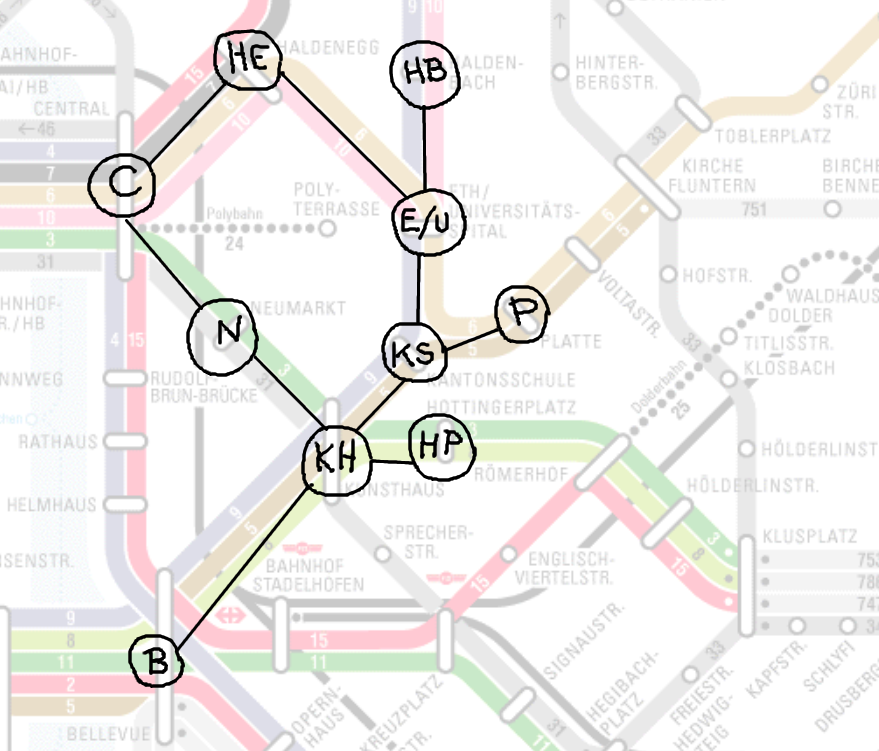
\includegraphics[width=\linewidth]{Pictures/Tram2.PNG}
    \caption{Ein Ausschnitt der Tram- und Buslinien in Zürich, als Graph formalisiert}
\end{figure}
Damit wir mit der Breitensuche beginnen können, müssen wir einen Startknoten auswählen. Wir wählen hier wie im Beispiel in der Einführung die Kantonsschule, also den Knoten {\bf{KS}} als Startknoten und schreiben ihn gleich auf eine Warteliste. Wir arbeiten also wiedereinmal mit dem ''First In, First Out''-Prinzip, denn wir gehen in jedem Schritt so vor, dass wir den ersten Knoten von der Warteliste entfernen und dafür seine noch unbesuchten Nachbarn der Warteliste anhängen. Im folgenden verwenden wir 3 Farben für die Knoten um die Breitensuche zu veranschaulichen. Blaue Knoten sind jene, die die Breitensuche noch nicht erreicht hat. Orange Knoten sind die besuchten Knoten, welche noch auf der Warteliste stehen. Graue Knoten sind jene, die wir bereits wieder von der Warteliste entfernt haben. Überlege anhand des Einführungsbeispiels, warum es so wichtig ist die besuchten Knoten zu markieren!

\begin{figure}[H]
    \centering
    \begin{subfigure}[h]{0.45\textwidth}
    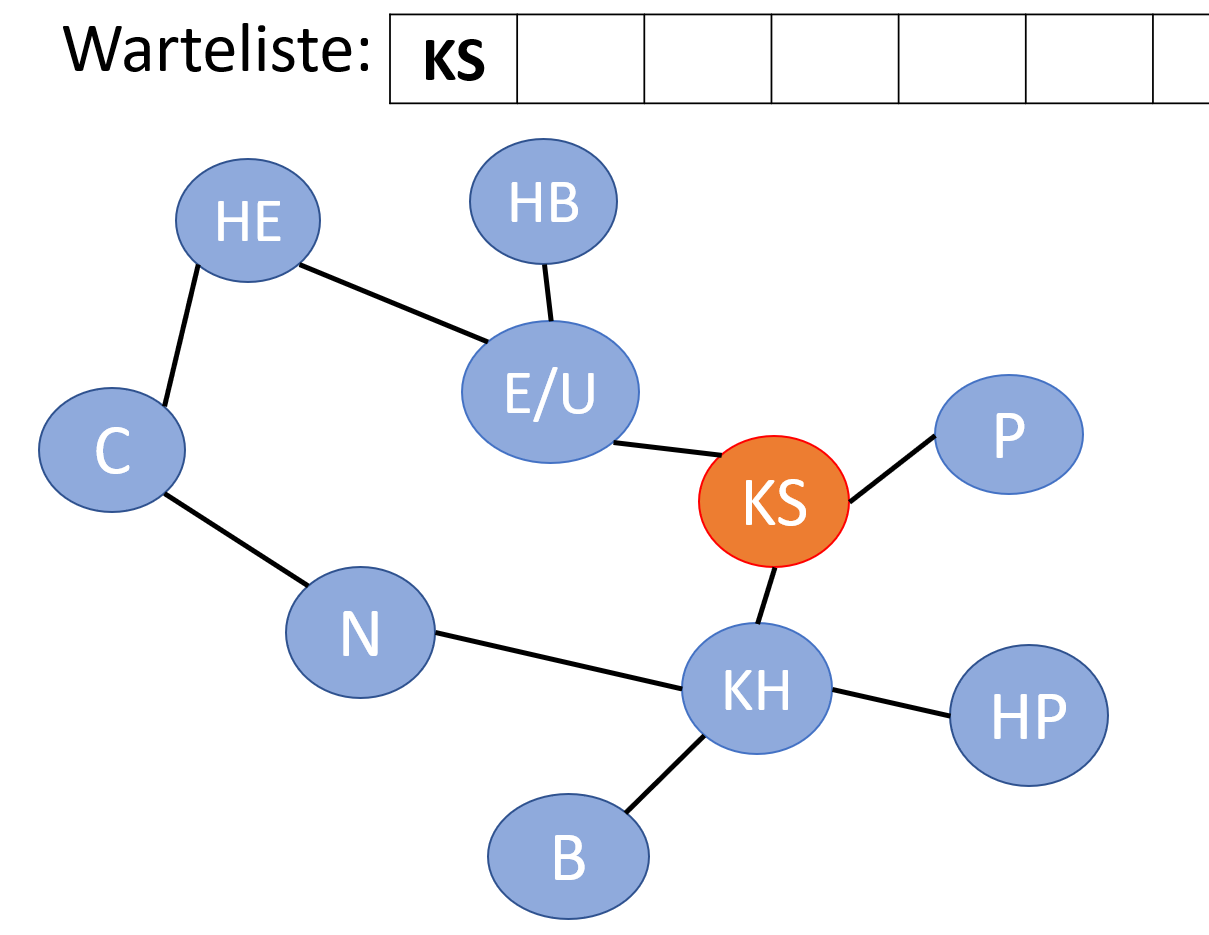
\includegraphics[width=\textwidth]{Pictures/BS/BFSB1.PNG}
    \caption{Die Breitensuche beginnt beim Startknoten {\bf{KS}}. Im ersten Schritt schreiben wir diesen auf unsere Warteliste und markieren ihn als besucht.}
    \label{fig:BS1}
    \end{subfigure}
    \vspace{5mm}
    \qquad
    \begin{subfigure}[h]{0.45\textwidth}
    \raggedleft
    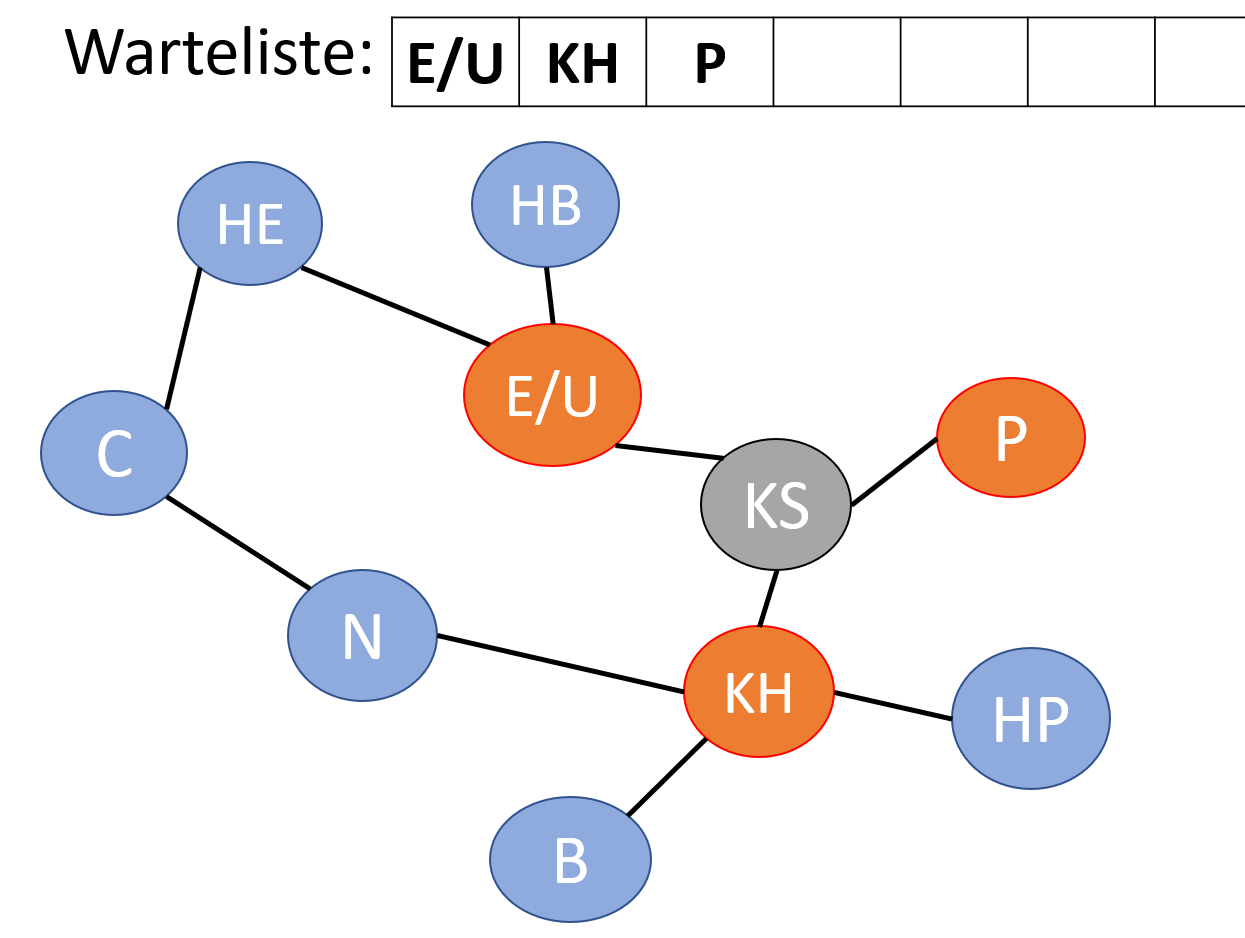
\includegraphics[width=\textwidth]{Pictures/BS/BFSB.PNG}
    \caption{Wir entfernen {\bf{KS}} aus der Warteliste und färben ihn darum grau. Als nächstes wollen wir die direkt benachbarten Haltestellen betrachten, wir schreiben sie also alphabetisch geordnet auf die Warteliste und markieren sie als besucht.}
    \label{fig:BS2}
    \end{subfigure}
    \vspace{5mm}
    \begin{subfigure}[h]{0.45\textwidth}
    \raggedright
    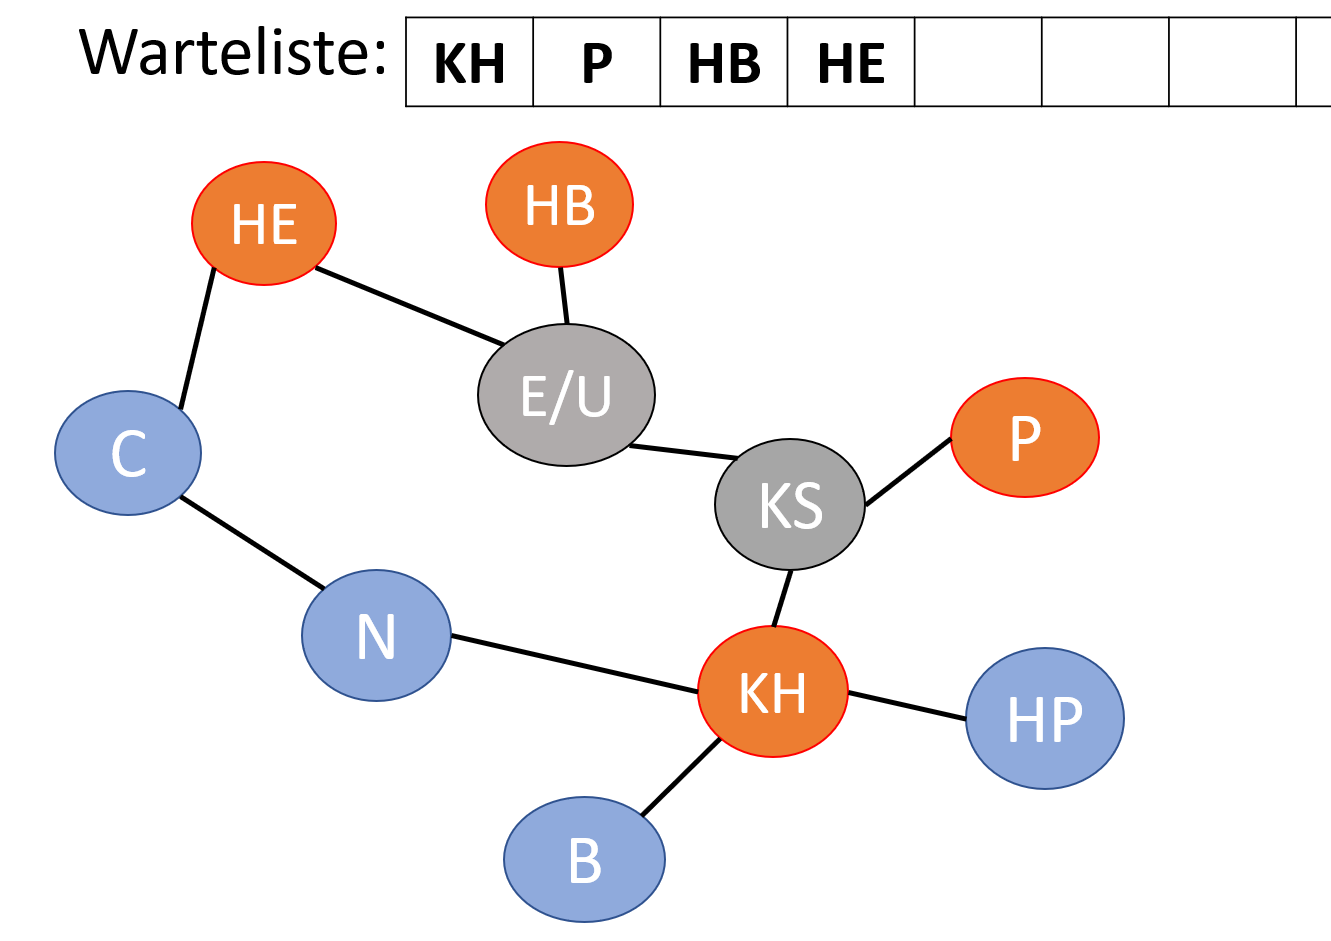
\includegraphics[width=\textwidth]{Pictures/BS/BFSB2.PNG}
    \caption{ Der erste Knoten auf der Warteliste war {\bf{E/U}}, wir entfernen ihn und hängen seine zwei unbesuchten Nachbarn {\bf{HB}} und {\bf{HE}} der Warteliste an.}
    \end{subfigure}
    \vspace{5mm}
    \qquad
    \begin{subfigure}[h]{0.45\textwidth}
    \raggedleft
    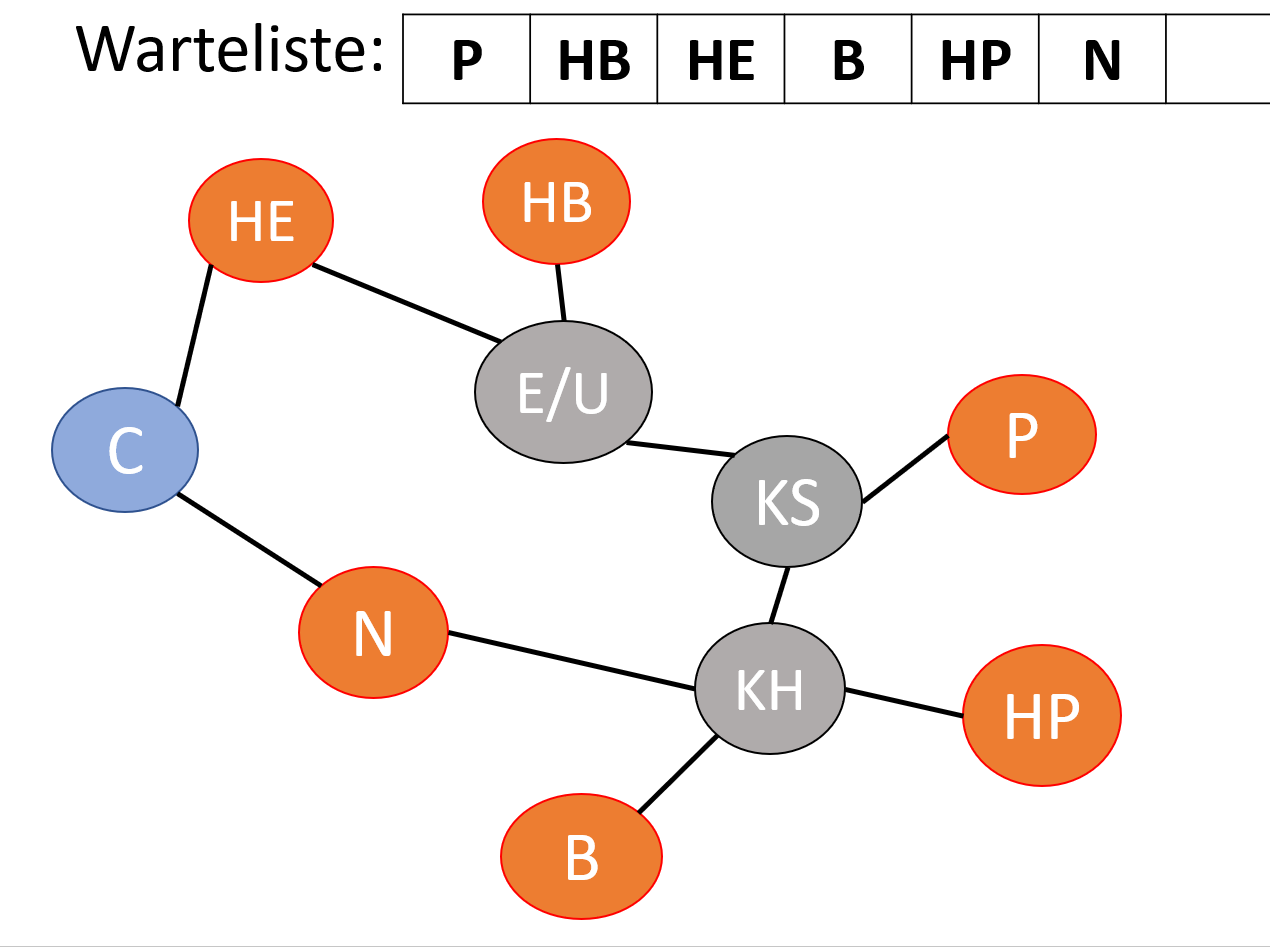
\includegraphics[width=\textwidth]{Pictures/BS/BFSB3.PNG}
    \caption{Der erste Knoten auf der Warteliste war {\bf{KH}}, wir entfernen ihn und hängen seine drei unbesuchten Nachbarn {\bf{B}}, {\bf{HP}} und {\bf{N}} der Warteliste an.} 
    \end{subfigure}
    \end{figure}
\begin{figure}[H]\ContinuedFloat
    \begin{subfigure}[h!]{0.45\textwidth}
    \centering
    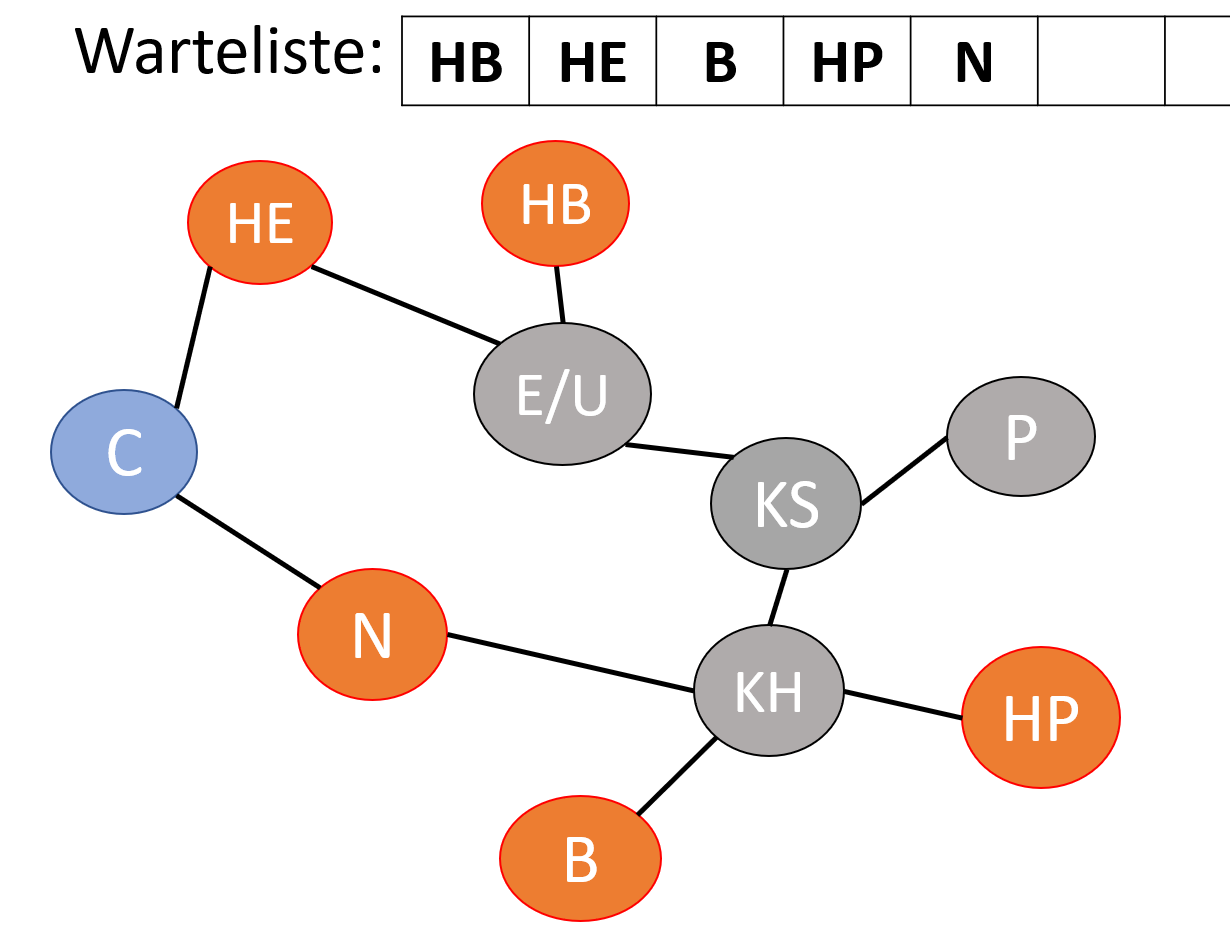
\includegraphics[width=\textwidth]{Pictures/BS/BFSB4.PNG}
    \caption{Als letzten Nachbarn von {\bf{KS}} können wir {\bf{P}} von der Warteliste entfernen. Er hat keine weiteren unbesuchten Nachbarn.} 
    \end{subfigure}
    \vspace{5mm}
    \qquad
    \begin{subfigure}[h]{0.45\textwidth}
    \centering
    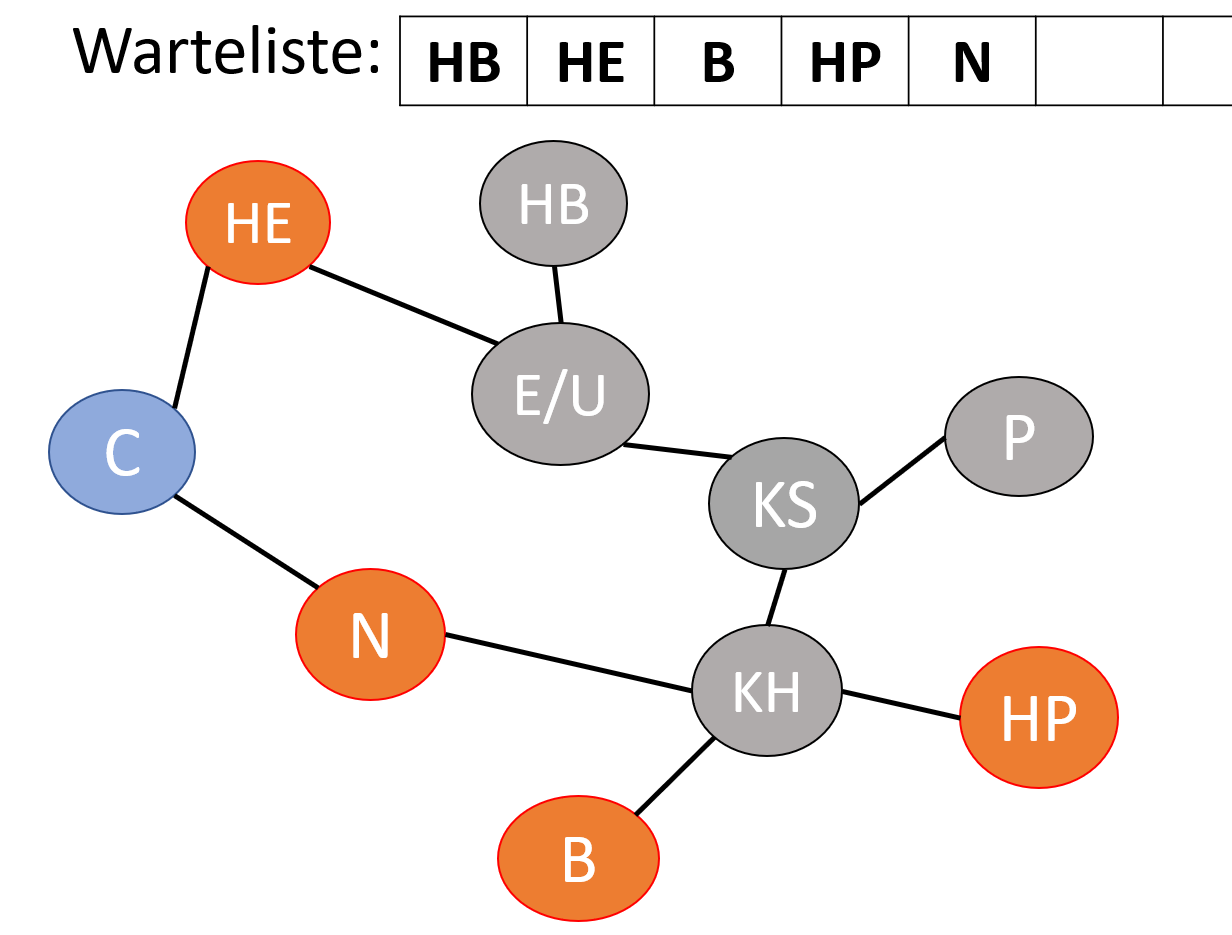
\includegraphics[width=\textwidth]{Pictures/BS/BFSB5.PNG}
    \caption{Als nächstes stehen in der Warteschlange die Nachbarn von {\bf{E/U}}. Wir entfernen zuerst {\bf{HB}} und müssen keine Knoten der Warteliste anhängen.}
    \end{subfigure}
    \vspace{5mm}
    \begin{subfigure}[h]{0.45\textwidth}
    \centering
    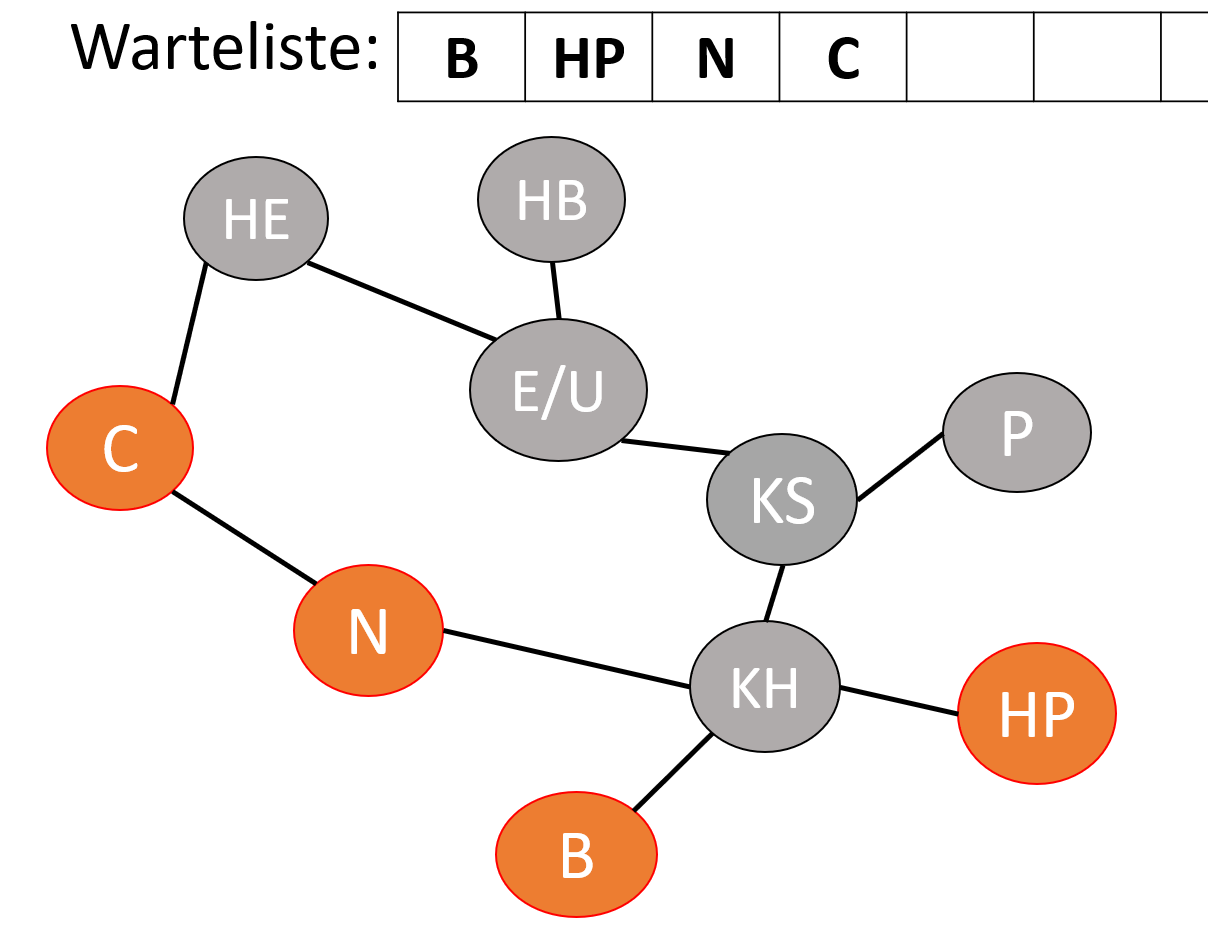
\includegraphics[width=\textwidth]{Pictures/BS/BFSB6.PNG}
    \caption{Wir entfernen {\bf{HE}} von der Warteliste, und hängen seinen unbesuchten Nachbarn {\bf{C}} der Warteliste an.}
    \end{subfigure}
    \qquad
    \begin{subfigure}[h]{0.45\textwidth}
    \centering
    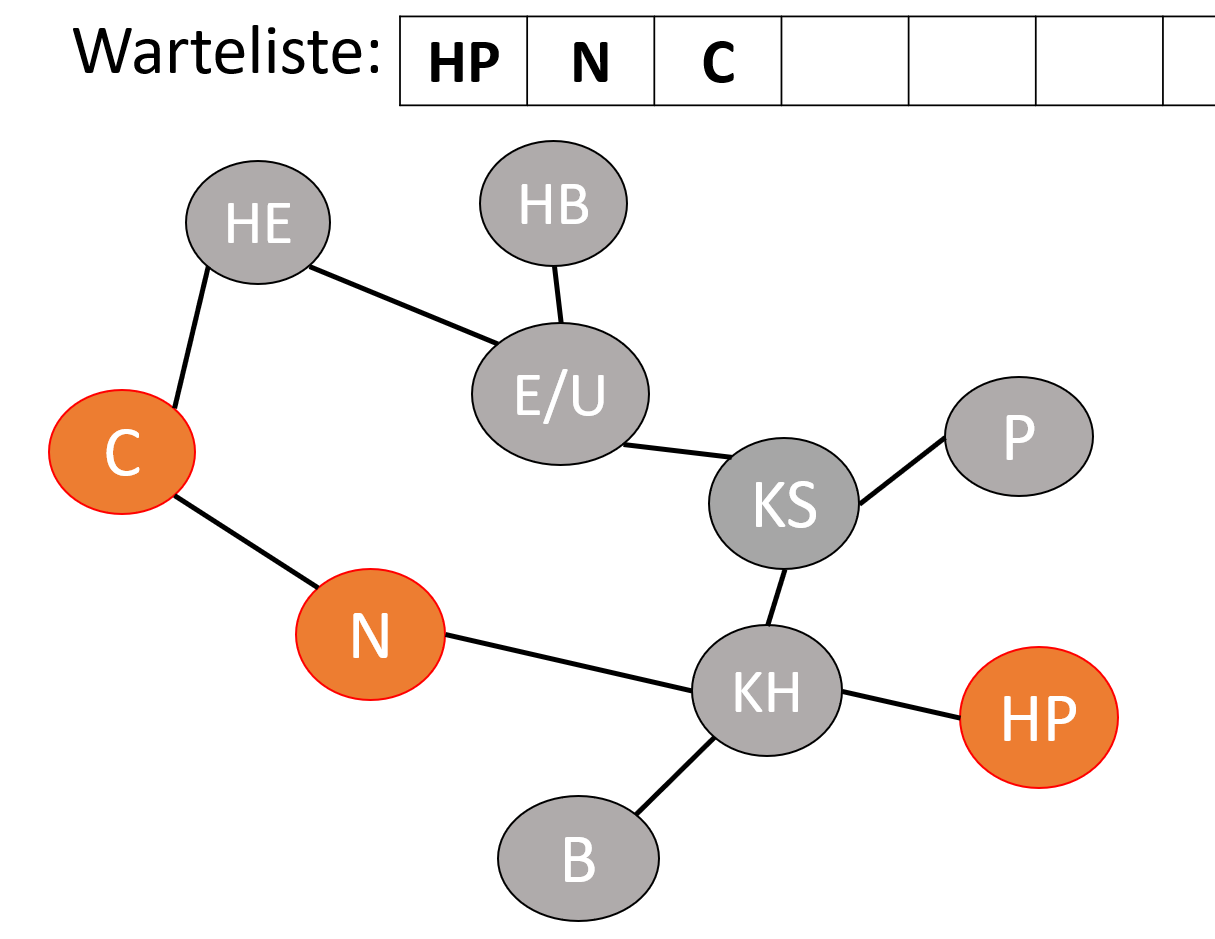
\includegraphics[width=\textwidth]{Pictures/BS/BFSB7.PNG}
    \caption{Wir entfernen {\bf{B}} aus der Warteliste. Der Knoten hat keine unbesuchten Nachbarn.}
    \end{subfigure}
\end{figure}
\begin{figure}[H]\ContinuedFloat
    \begin{subfigure}[h]{0.45\textwidth}
    \centering
    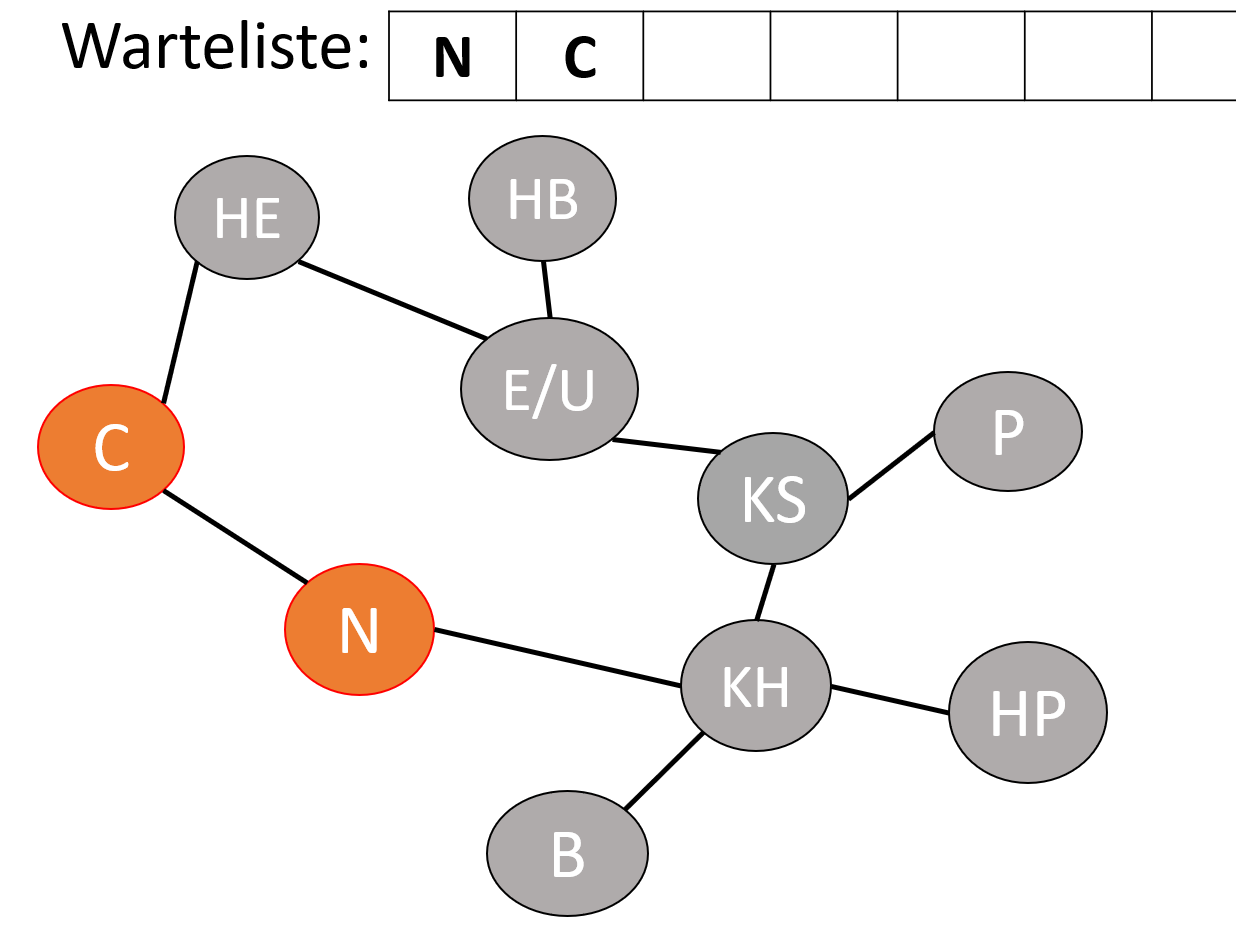
\includegraphics[width=\textwidth]{Pictures/BS/BFSB8.PNG}
    \caption{Wir entfernen {\bf{HP}} aus der Warteliste. Der Knoten hat keine unbesuchten Nachbarn.}
    \end{subfigure}
    \qquad
    \begin{subfigure}[h]{0.45\textwidth}
    \centering
    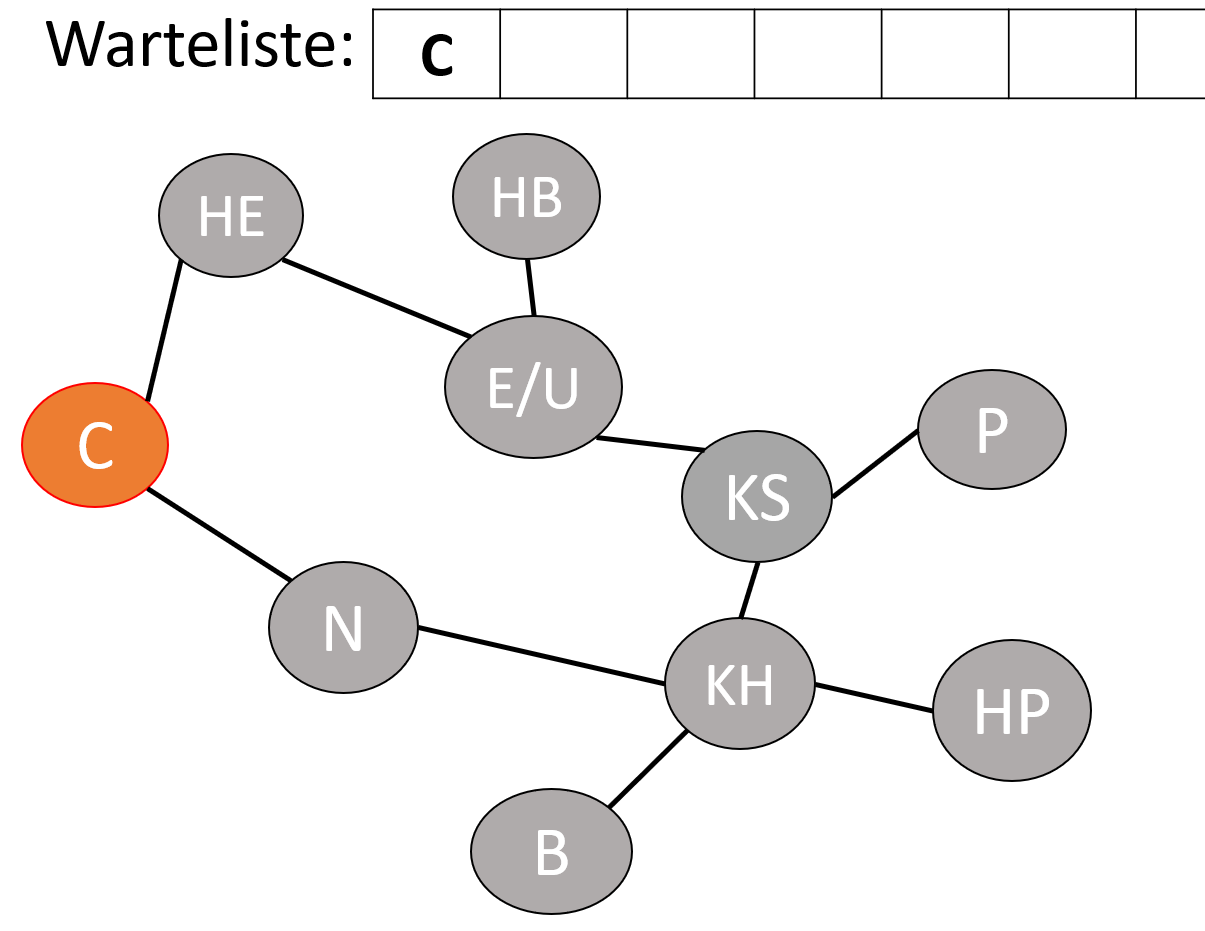
\includegraphics[width=\textwidth]{Pictures/BS/BFSB9.PNG}
    \caption{Als letzten Nachbarn von {\bf{KH}} können wir {\bf{N}} von der Warteliste entfernen. Die Nachbarn von {\bf{N}} sind alle bereits als besucht markiert. }
    \end{subfigure}
\end{figure}
\begin{figure}[H]\ContinuedFloat
     \centering
     \begin{subfigure}[h]{0.45\textwidth}
    \centering
    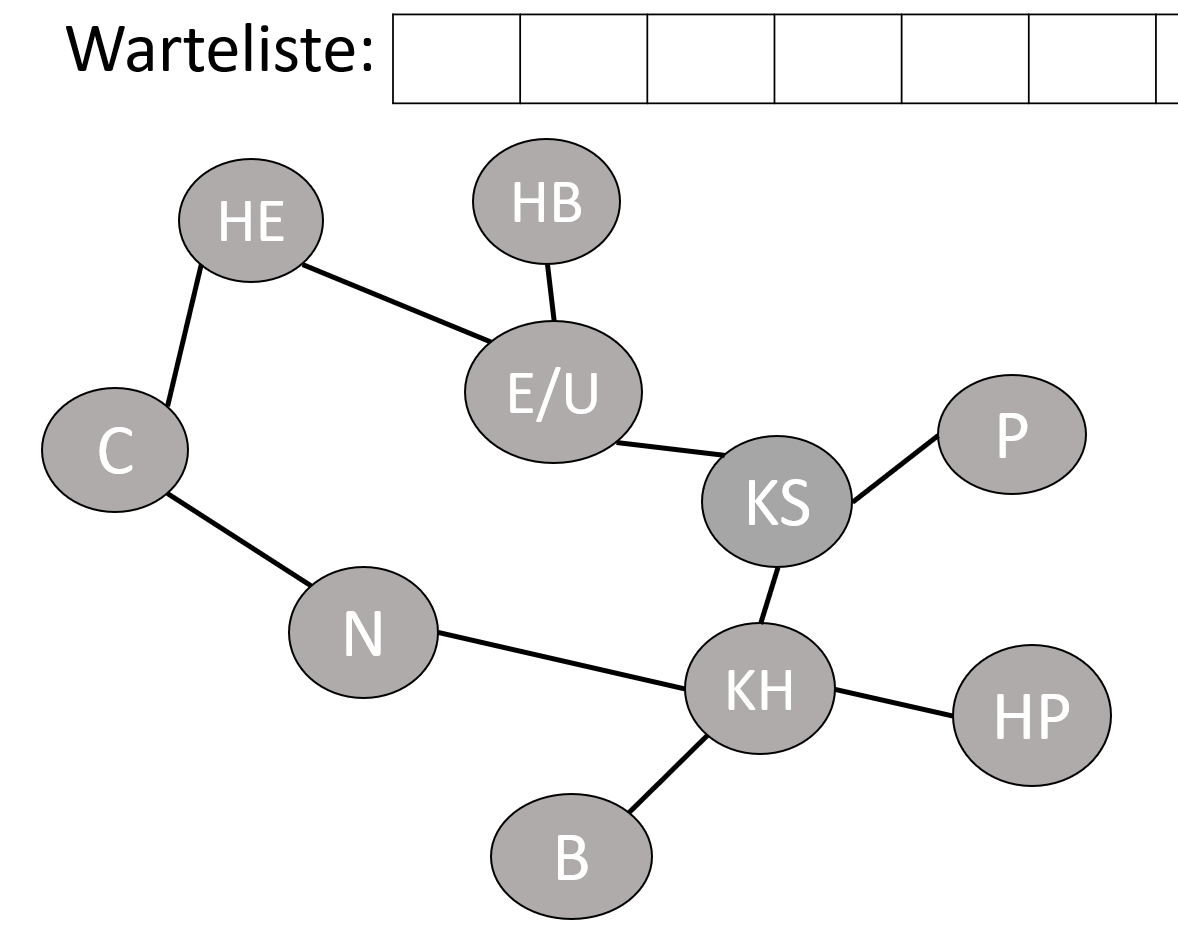
\includegraphics[width=\textwidth]{Pictures/BS/BFSB10.PNG}
    \caption{Zuletzt entfernen wir {\bf{C}} aus der Warteliste. Seine Nachbarn wurden alle bereits einmal besucht und die Warteliste ist jetzt leer. Der Algorithmus endet also an dieser Stelle.}
    \end{subfigure}
\end{figure}
Die Breitensuche besucht die Knoten also in der Reihenfolge 
$$ \text{ \bf{KS,E/U,KH,P,HB,HE,B,HP,N,C}} $$

\subsection{Der Algorithmus in Worten}
Wir wollen nun den Suchalgorithmus, welchen wir oben graphisch an einem Beispiel aufgezeichnet haben, allgemein formalisieren. In einer ersten Version geben wir dem Algorithmus keine Abbruchsbedingung, das heisst die Breitensuche läuft weiter, bis alle möglichen Knoten einmal besucht wurden. Um uns jeweils zu merken, welche Knoten wir als nächstes betrachten wollen, verwenden wir eine Warteliste. Um uns zu merken, welche Knoten wir bereits betrachtet haben, markieren wir diese als besucht. So können wir vermeiden, dass ein Knoten mehrmals bearbeitet wird.\\

 \noindent {\bf{Input:}} Ein Graph $G=(V,E)$ und ein Startknoten $s \in V$.

\noindent {\bf{Output:}} Die Knoten von $G$ aufsteigend geordnet nach Abstand zum Startknoten $s$.

\begin{enumerate}
    \item Schreibe den Startknoten $s$ auf die Warteliste und markiere ihn als besucht.
    \item Entferne den ersten Knoten von der Warteliste und prüfe für jeden Nachbarn, ob er bereits als besucht markiert wurde.
    \item Falls nicht, hänge ihn der Warteliste an und markiere ihn als besucht.
    \item Wiederhole die Schritte 2 und 3 bis keine Knoten mehr auf der Warteliste sind.
\end{enumerate}

\begin{aufgabe} \label{newinitial}
In welcher Reihenfolge besucht die Breitensuche die Haltestellen, wenn wir statt bei der Kantonsschule beim Bellevue starten?
\end{aufgabe}

\begin{aufgabe} \label{directed}
Wir betrachten immer noch den Graphen in Abbildung \ref{fig:BS1}. Nun
treten bei verschiedenen Trams technische Störungen auf, so dass die Strecken Bellevue - Platte und Central - Hottingerplatz jeweils nur noch in dieser einen Richtung befahren werden können. Zeichne den gerichteten Graphen (mit den gleichen 10 Knoten), der zu dieser Situation passt. In welcher Reihenfolge besucht die Breitensuche jetzt die Knoten, wenn wir wieder beim Bellevue starten? 
\end{aufgabe}


Alice und Bob spielen das Wikipedia-Spiel. Es funktioniert wie folgt: Alice gibt Bob zwei Wikipedia-Artikel vor und dieser muss durch das Klicken von möglichst wenigen Links von einem Artikel zum anderen kommen. Wir können Wikipedia als Graphen darstellen, indem wir für jeden Artikel einen Knoten zeichnen und für einen Link in Artikel $A$ zu Artikel $B$ eine gerichtete Kante von $A$ nach $B$. Der tatsächliche Graph von allen deutschen Wikipedia-Artikeln hat so fast 2.5 Millionen Knoten und noch viel mehr Kanten. Wir betrachten nur einen sehr kleinen Ausschnitt davon mit den folgenden Artikeln:
\begin{multicols}{2}
\begin{itemize}
    \item {\bf{B}}: Bellevue
    \item {\bf{BS}}: Breitensuche
    \item {\bf{D}}: Deutschland
    \item {\bf{E}}: Eisenbahn
    \item {\bf{G}}: Graph
    \item {\bf{K}}: Knoten
    \item {\bf{L}}: Laufzeit
    \item {\bf{S}}: Schweiz
    \item {\bf{SBZ}}: Strassenbahn Zürich
    \item {\bf{U-B}}: U-Bahn
    \item {\bf{Z}}: Zürich
\end{itemize}

\end{multicols}
mit dem zugehörigen gerichteten Graphen:
\begin{figure}[h!]
    \centering
    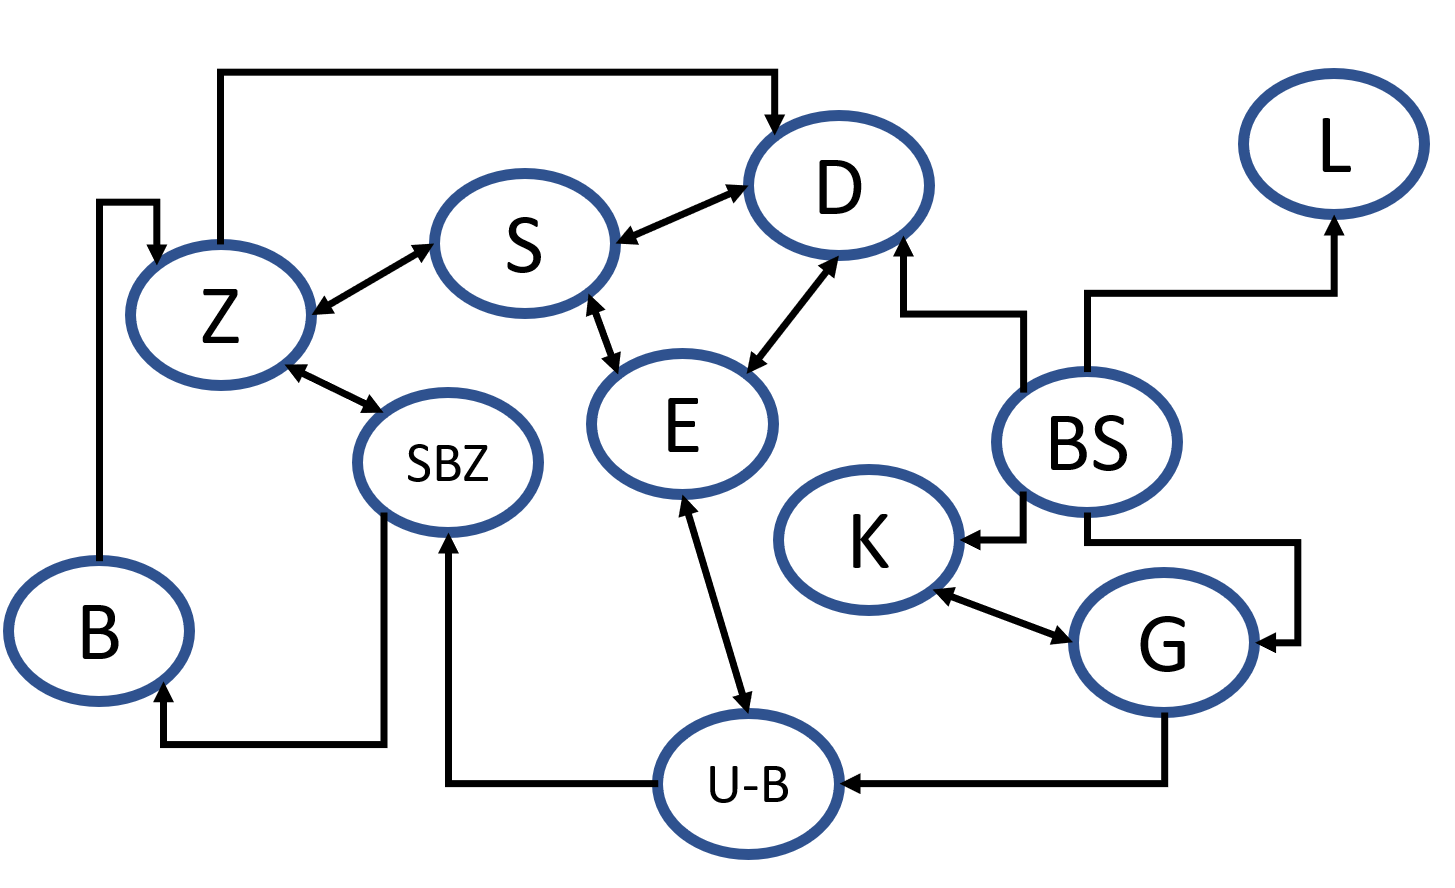
\includegraphics[scale=0.5]{Pictures/Wikipedia.PNG} 
    \caption{Die Verlinkung von Wikipedia-Artikeln als Graph.}
    \label{fig:my_label}
\end{figure}

\begin{aufgabe} \label{Wikipedia}
Alice sagt zu Bob: ''Öffne den Wikipedia-Artikel über die Breitensuche und finde den Artikel über die Strassenbahnen von Zürich.'' Wenn Bob nur die 11 aufgelisteten Artikel zur Verfügung hat, kann er dann den gewünschten Artikel erreichen? Verwende die Breitensuche um die Frage zu beantworten.
\end{aufgabe}

In Aufgabe \ref{Wikipedia} haben wir eine Abbruchsbedingung in Form eines gesuchten Knotens. Wir können also der Breitensuche als Input zusätzlich zum Graphen und Startknoten noch einen Zielknoten geben und den Algorithmus abbrechen, sobald der Zielknoten als besucht markiert wurde.

Jetzt wäre es natürlich schön, wenn wir den Algorithmus so abändern könnten, dass er uns zusätzlich sagt, wieviele Klicks Bob mindestens braucht und was eine mögliche optimale Lösung wäre. Doch bevor wir dieses Problem lösen, wollen wir zuerst die Breitensuche in Python implementieren.

\subsection{Der Algorithmus in Python}
Wir wollen ein Programm für die Breitensuche schrieben und dieses gleich an unserem Tramlinienbeispiel testen.
Da wir uns bei der Breitensuche jeweils für jeden Knoten alle seine Nachbarn merken (bzw. auf die Warteliste schreiben) müssen, bietet es sich an die ''Liste der Nachbarn''- Darstellung für die Graphen zu verwenden.
In Python implementieren wir einen Graphen also am besten als eine Menge von Listen. Der Graph in Abbildung \ref{fig:BS1} wäre zum Beispiel:

\begin{figure}[H]
    \centering
    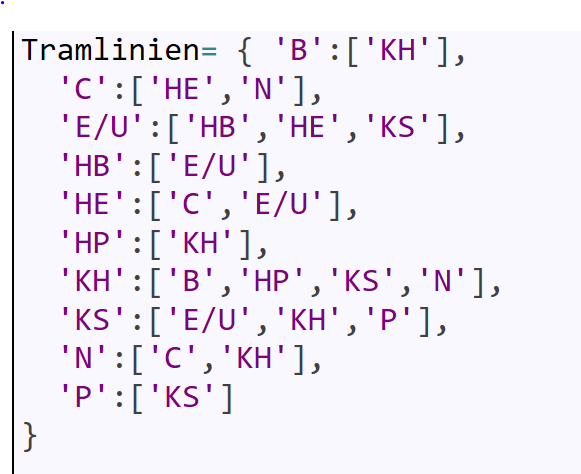
\includegraphics[scale=0.8]{Pictures/ListeDerNachbarn.PNG}
    \caption{Tramliniengraph in der ''Liste der Nachbarn''-Darstellung}
    \label{fig:Tram2}
\end{figure}

Tippe das Programm in Abbildung \ref{fig:Breitensuche} ab. Vergleiche die Ausgabe mit der Reihenfolge der Knoten die wir im Abschnitt 2.1 gefunden haben.

\begin{figure}[H]
    \centering
    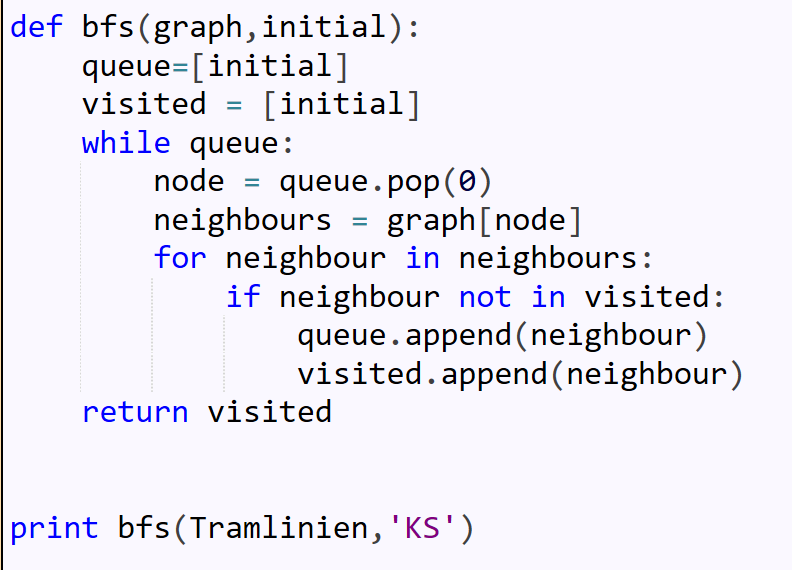
\includegraphics[scale=0.8]{Pictures/Breitensucheprog.PNG}
    \caption{Breitensuche in Python}
    \label{fig:Breitensuche}
\end{figure}

Wir nennen das Programm ''bfs'' für ''breadth first search'' (englischer Name der Breitensuche). 

\begin{aufgabe} \label{ProgFragen} Beantworte folgende Fragen zum Programm in Abbildung \ref{fig:Breitensuche}
\begin{itemize} 
    \item Wofür brauchen wir die Listen ''queue'' und ''visited''?
    \item Welche Zeilen im Programm entsprechen welchem Schritt des Algortihmus in Abschnitt 2.1?
\end{itemize}
\end{aufgabe}

\paragraph{Die Laufzeit} hängt bei einem Algorithmus für Graphen davon ab, wieviele Knoten und Kanten dieser hat. Falls die Breitensuche durch den ganzen Graphen $G=(V,E)$ läuft, so durchlaufen wir die while-Schlaufe für jeden Knoten einmal, also insgesammt $|V|$-mal. In der for-Schlaufe betrachten wir jeweils jede ausgehende Kante, insegsamt durchlaufen wir sie also maximal (bei einem ungerichteten Graphen) $2|E|$-mal. Die Laufzeit der einzelnen Schritte ist immer $\mathcal{O}(1)$. Wir erhalten eine Gesamtlaufzeit von $\mathcal{O}(|V|+|E|)$. Die Zeit, welche der Computer benötigt um die Breitensuche durchzuführen, wächst also linear in der Anzahl der Knoten und Kanten des Graphens an.

\paragraph{Der Speicherplatzverbrauch} der Breitensuche ist $\mathcal{O}(|V|)$ da wir alle bisher besuchten Knoten speichern. Sobald du mehrere Algorithmen für Graphen kennst kannst du sie anhand ihrer Laufzeiten und ihrem Speicherplatzverbrauch miteinander vergleichen.

\begin{aufgabe}  \label{WikiProgAufg} {\bf{*}}
Ändere das Programm ''bfs'', so dass es abbricht sobald ein gesuchter Knoten gefunden wurde und überprüfe damit deine Lösung von Aufgabe \ref{Wikipedia}. Nenne das neue Programm ''bfs\_goal''.
\end{aufgabe}

\paragraph{Lernaufgabe}
Alice und Bob haben eine Datenbank ('Familien') zur Verfügung in welcher für jeden Menschen jeweils die Eltern und die Kinder aufgeführt sind. Sie geht 6 Generationen zurück. Nun fragen sie sich ob sie eine gemeinsame Ur-ur-ur-ur-Grossmutter haben. 
\begin{enumerate}
    \item Wie können sie die Daten als ungerichteten Graphen darstellen?
    \item Wie können sie die Antwort zu ihrer Frage mit Hilfe des Programms ''bfs\_goal'' finden? Beschreibe deine Idee in Worten. (noch nicht programmieren)
\end{enumerate}
Nun wollen sie ein Programm welches ihnen statt der Liste aller besuchten Knoten als Ausgabe einfach mitteilt ob sie eine gemeinsame Ur-ur-ur-ur-Grossmutter haben und zwar in Form einer Ausage wie: '' Der Startknoten und der Endknoten sind in \dots '' oder ''Der Startknoten und der Endknoten sind nicht in \dots''
\begin{enumerate}[resume]
    \item Was kommt in die Lücke des gewünschten Outputs?
    \item Schreibe das Programm und teste es an einem kleinen Graphen.
\end{enumerate}

\subsection{Kontrollfragen}
\begin{enumerate}
    \item Wie würdest du einem Mitschüler, welcher diesen ersten Teil der Stunde verpasst hat, in wenigen Sätzen erklären, was die Breitensuche ist?
    \item Du kennst bereits viele verschiedene Zusammenhänge, welche sich als Graphen darstellen lassen. Überlege dir eine ''Alltagssituation'', bei der du die Breitensuche verwenden könntest.
\end{enumerate}
Welche der folgenden Schüler haben recht? Welche nicht? Begründe!
\begin{enumerate}[resume]
    \item David sagt:''Es gibt bestimmt Graphen bei denen ein Knoten im Laufe der Breitensuche mehr als einmal in der Warteliste auftaucht.''
    \item Fred behauptet: ''Ob ich einen bestimmten Knoten in einem zusammenhängeden Graphen finden kann hängt nicht davon ab welchen Startknoten ich gewählt habe.''
    \item * Gregory meint: '' Ich kann einen zusammenhängenden Graphen mit beliebig vielen Knoten zeichnen und den Startknoten so wählen, dass nie mehr als ein Knoten auf der Warteliste steht.
\end{enumerate}

\newpage
\newpage

\section{Kürzeste Pfade}\label{kuerzeste_pfade}
Die Breitensuche ist nicht nur ein Verfahren, um Knoten in einem Graphen systematisch aufzulisten. Dank der speziellen Reihenfolge, in der die Knoten besucht werden (zuerst die direkten Nachbarn, dann dessen Nachbarn und so weiter), sind wir sicher, dass wir jeden erreichbaren Knoten über einen kürzesten Pfad erreichen. In diesem Abschnitt werden wir den Algorithmus, den wir im vorherigen Abschnitt kennengelernt haben, so abändern und erweitern, dass wir zuerst den Abstand zwischen zwei Knoten in einem Graphen berechnen können und dann sogar die Knoten auf dem kürzesten Pfad auflisten.

\subsection{Die Länge des kürzesten Pfades}

Wie wir schon wissen, ist der \textbf{Abstand} zwischen zwei Knoten definiert als die Länge des kürzesten Pfades zwischen diesen zwei Knoten. Ein \textbf{Pfad} ist eine Folge von Knoten, die, wie eine Kette, eine Kante zum vorherigen und zum nächsten Knoten haben. Die \textbf{Länge} eines Pfades ist die Anzahl Kanten auf dem Pfad.

\begin{beispiel}
Betrachte folgenden Graphen.
\begin{figure}[H]
\centering
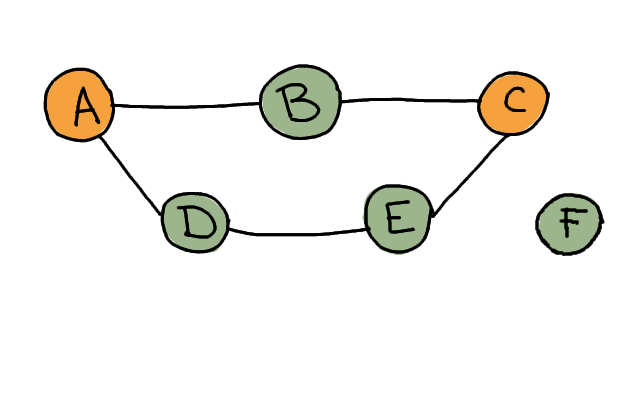
\includegraphics[width=0.5\linewidth]{Pictures/SP/abstand_def.png} 
\end{figure}
Der Abstand zwischen \textbf{A} und \textbf{C} ist \(2\). Zwischen \textbf{A} und \textbf{C} gibt es zwei Pfade: \textbf{ABC} und \textbf{ADEC}. Der Pfad \textbf{ABC} ist der kürzeste und hat zwei Kanten, somit ist der Abstand zwischen \textbf{A} und \textbf{C} \(2\).

Bevor du weiterliest, überlege kurz, was der Abstand zwischen \textbf{A} und \textbf{F} sein könnte.

Beobachte, dass es zwischen \textbf{A} und \textbf{F} gar keinen Pfad gibt. Sie sind nicht verbunden. In einem solchen Fall sagen wir, dass der Abstand \(\infty\) (unendlich) ist.
\end{beispiel}

\begin{aufgabe}\label{aufgabe_abstand_ex}
Betrachte folgenden Graphen.
\begin{figure}[H]
    \centering
    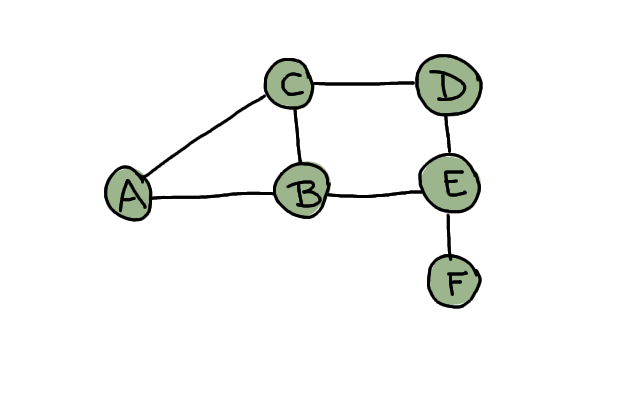
\includegraphics[width=0.5\textwidth]{Pictures/SP/abstand_ex.png} 
    \label{fig:abstand_ex}
\end{figure}
Was ist der Abstand zwischen \textbf{A} und \textbf{F}?
Was ist der Abstand zwischen \textbf{C} und \textbf{E}?
\end{aufgabe}
\begin{aufgabe}\label{aufgabe_abstand}
\begin{enumerate}[(a)]
\item \label{aufgabe_abstand_k5} Zeichne einen vollständigen Graphen mit 5 Knoten. Was ist die Länge des kürzesten Pfades zwischen zwei beliebigen Knoten?
\item \label{aufgabe_abstand_gitter23} Zeichne einen Gittergraphen mit 2 mal 3 Knoten. Welche zwei Knoten sind am weitesten auseinander? Bestimme den Abstand (die Länge des kürzesten Pfades) zwischen diesen zwei Knoten.
\item \label{aufgabe_abstand_kreis6} Zeichne einen Kreis mit 6 Knoten. Welche zwei Knoten sind am weitesten auseinander? Wie weit sind sie voneinander entfernt?
\end{enumerate}
\end{aufgabe}

\subsubsection*{Das Wikipedia-Spiel}
Als wir den Breitensuchealgorithmus in Worten definiert hatten, haben wir das Wikipedia-Spiel kennengelernt. Alice gibt Bob zwei Wikipediaartikel vor und er muss vom Startartikel aus auf Links klicken, bis er auf den Zielartikel stosst. Das Ziel ist mit möglichst wenigen Klicks auszukommen.

Der Wikipedia-Graph ist nicht so übersichtlich und regelmässig, wie die Graphen, die wir gerade gesehen haben. Um den kürzesten Pfad zwischen zwei Artikel zu finden, muss Bob systematisch vorgehen. 
\begin{figure}[H]
    \centering
    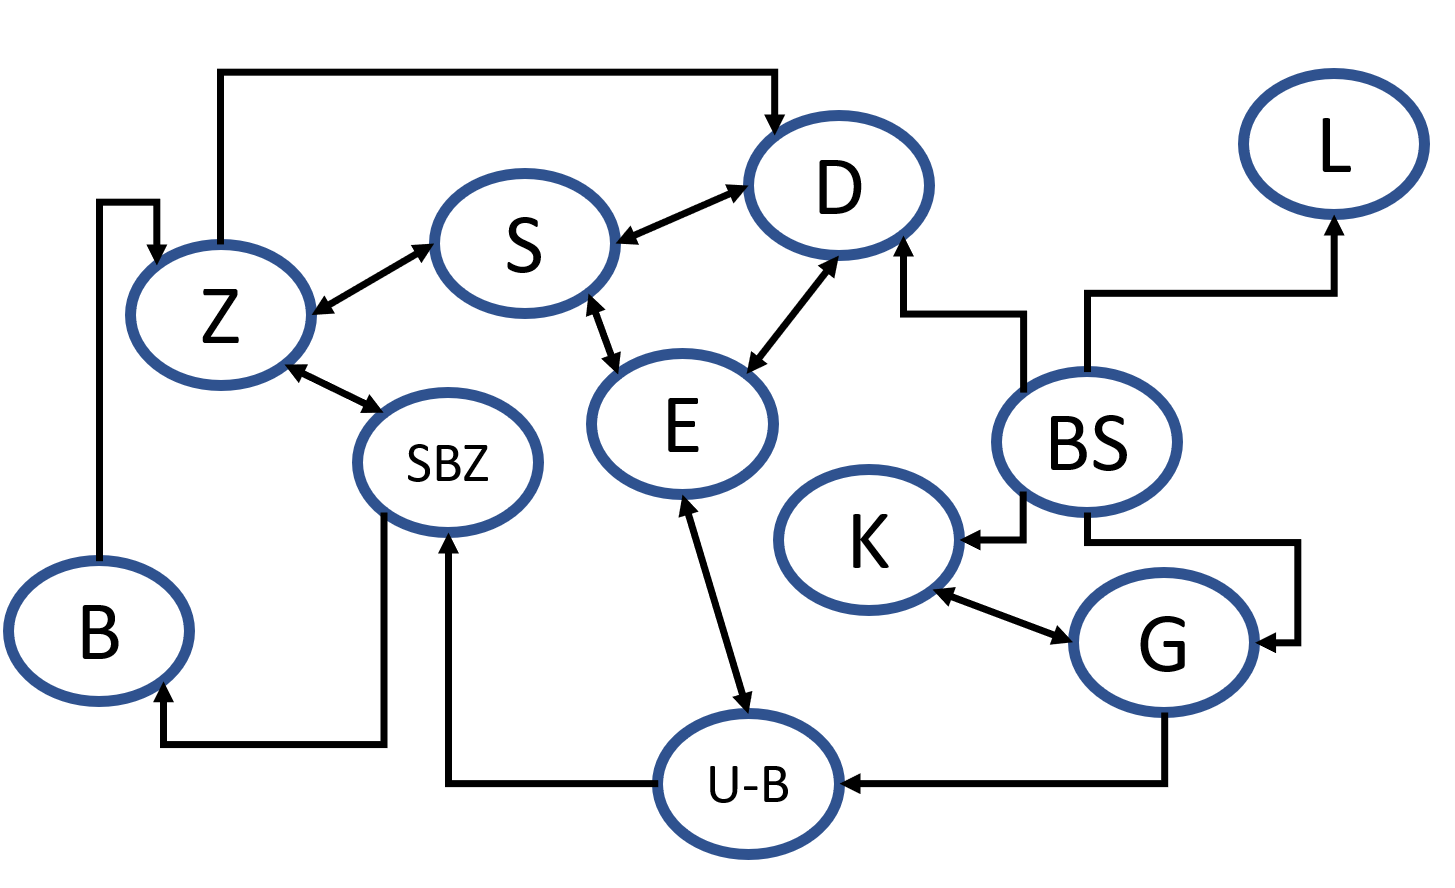
\includegraphics[width=0.7\textwidth]{Pictures/Wikipedia.PNG} 
    \caption{Die Verlinkung von Wikipedia-Artikeln als Graph.}
    \label{fig:wikipedia_graph}
\end{figure}

Wenn er nach dem Breitensuchealgorithmus vorgeht, wird er den Startartikel im Browser aufmachen (\textit{Breitensuche}, in unserem Beispiel von vorher) und dann jeden Link (\textit{Deutschland}, \textit{Graph}, \textit{Laufzeit}, \textit{Knoten}) in einem neuen Tab öffnen und anschliessend den Tab mit der Breitensuche schliessen. All die Artikel, die er jetzt im Browser offen hat, sind ein Klick vom Breitensucheartikel entfernt. Jetzt kann er dasselbe für den zuerst geöffneten noch offenen Tab (\textit{Deutschland}) tun. Er muss sich einfach merken, dass die neugeöffneten Tabs (\textit{Eisenbahn}, \textit{Schweiz}) sind jetzt 2 Klicks entfernt: Ein Klick mehr als die Seite, woher er kommt (\textit{Deutschland}). Er kann einfach für jeden Artikel aufschreiben, wie viele Klicks er vom Breitensucheartikel entfernt ist. Jeder nicht besuchte benachbarte Artikel wird ein Klick weiter sein.

\begin{aufgabe}\label{aufgabe_wikipedia_spiel}
Alice und Bob spielen das Wikipedia-Spiel auf den Graphen in Abbildung \ref{fig:wikipedia_graph}. Bob startet bei \textbf{BS} und muss in möglichst wenig Klicks \textbf{SBZ} erreichen. Helfe Bob herauszufinden, wie viele Klicks er braucht. Wie musst du den Breitensuchealgorithmus modifizieren, um die minimale Anzahl Klicks zu ermitteln? Führe deinen modifizierten Breitensuchealgorithmus auf diesen Graphen aus. Wie sehen in jedem Schritt \texttt{queue} und \texttt{visited} aus? Wo schreibst du die Abstände zwischen dem Startknoten und jedem besuchten Knoten auf?
\end{aufgabe}

\subsubsection*{Abstand zwischen zwei Knoten in Python ausrechnen}
Die Aufgabe \ref{aufgabe_wikipedia_spiel} hat mehrere möglichen Lösungen. Wir werden eine der Varianten in Python implementieren. In dieser Variante werden wir die Abstände genau dort speichern, wo wir sie brauchen: in der Warteschlange. Grundsätzlich gibt es zwei grosse Änderungen:
\begin{enumerate}
    \item Die Warteschlange enthält nicht nur Knoten, sondern auch deren Abstand vom Startknoten.
    \item Das Programm gibt anstatt von der Liste aller besuchten Knoten den Abstand zwischen Start- und Zielknoten zurück.
\end{enumerate}

\begin{figure}[H]
    \centering
    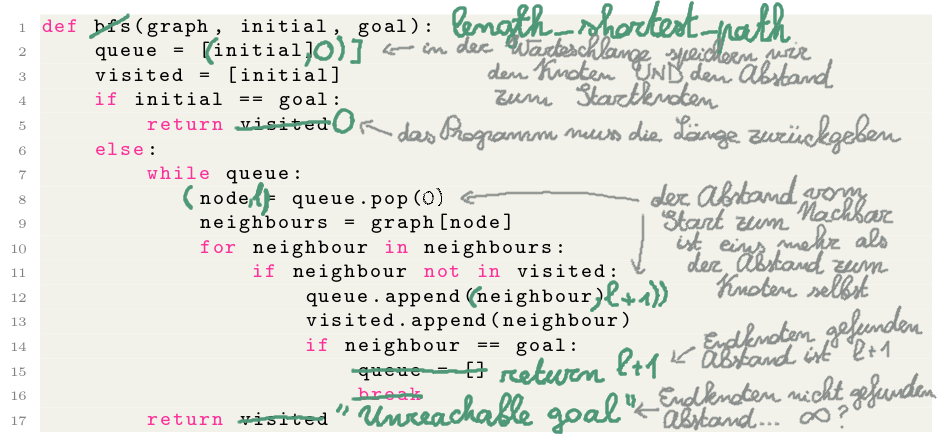
\includegraphics[width=\textwidth]{Pictures/SP/bfs_goal-to-length.png}
    \caption{Programm, das einen bestimmten Knoten sucht, in ein Programm umschreiben, das den Abstand zwischen Start- und Zielknoten findet.}
    \label{fig:bfs_goal_to_length}
\end{figure}

\begin{lstlisting}[language=Python, caption={Programm, das den Abstand zwischen \texttt{initial} und \texttt{goal} berechnet.}, label={lst:length_shortest_path}]
def length_shortest_path(graph, initial, goal):
    queue = [(initial, 0)]
    visited = [initial]
    if initial == goal:
        return 0
    else:
        while queue:
            (node, length) = queue.pop(0)
            new_length = length + 1
            neighbours = graph[node]
            for neighbour in neighbours:
                if neighbour not in visited:
                    queue.append((neighbour, new_length))
                    visited.append(neighbour)
                    if neighbour == goal:
                        return new_length
        return "There is no path between initial and goal in the given graph"
\end{lstlisting}

\begin{framed}
\paragraph{\textcolor{blue-violet}{Was haben wir gelernt:}}
Um die \textbf{Länge des kürzesten Pfades} zwischen Start- und Zielknoten in einem Graphen zu finden, können wir eine abgeänderte Version vom Breitensuchealgorithmus verwenden. Wie in der normalen Breitensuche, verwenden wir eine Warteschlange, um die zu besuchenden Knoten zu speichern. Aber in dieser Version enthält die Warteschlange nicht nur die zu besuchende Knoten, sondern auch deren \textbf{Abstand vom Startknoten}. Wir können diesen Abstand sehr einfach berechnen: Die Nachbarn eines Knotens sind \textbf{um \(1\) weiter}, als der Knoten selbst.

Wenn die Breitensuche abbricht, weil der Zielknoten gefunden wurde, dann können wir dessen Abstand aus der Warteschlange einfach ablesen. Die Breitensuche kann aber auch terminieren, ohne den Zielknoten gefunden zu haben. Wenn der Zielknoten im Graphen existiert, aber vom Startknoten nicht erreicht werden kann, dann sagen wir, dass der Start- und Zielknoten zu unterschiedlichen \textbf{Zusammenhangskomponenten} gehören.
\end{framed}


\subsubsection*{\textcolor{blue-violet}{Teste dich selber}}
\begin{aufgabe}\label{laenge_kontrollfragen}
Beantworte folgende Fragen.
\begin{enumerate}[(a)]
\item Wie definiert man den Abstand zwischen zwei Knoten in einem Graphen?
\item Was hat die Breitensuche mit dem Abstand zwischen zwei Knoten zu tun?
\item Gregory behauptet: ''Wenn die Breitensuche terminiert, ohne den Zielknoten gefunden zu haben, dann ist der Zielknoten nicht im Graphen enthalten''. Hat er recht? Begründe deine Antwort.
\item Welche zusätzliche Informationen müssen wir während der Breitensuche speichern, um die Länge des kürzesten Pfades zwischen Start- und Zielknoten berechnen zu können?
\end{enumerate}
\end{aufgabe}


\paragraph{Über wie vielen Ecken kennt jeder jeden?}
Alice hat gehört, dass jeder jeden im Schnitt über 6,6 Ecken kennt. Das heisst, jede zwei Menschen auf der Welt sind über höchstens 7 Kontaktpersonen bekannt. Alice ist von dieser Theorie sehr begeistert und möchte herausfinden, über wie vielen Ecken sie eine Person kennt, die schon Mal von einem Panda gebissen worden ist.

\begin{aufgabe}\label{aufgabe_panda_gebissen}
Hier ist eine Beschreibung von den Freundschaften von Alice und ihren Freunden.
\begin{displayquote}
Bob ist der beste Freund von Alice. Bob kennt ausserdem Charlie und David. Charlie, Elisabeth und Fred sind sehr eng befreundet und essen zusammen Kuchen jedes Wochenende. Fred und Alice kennen beide Gregory. Gregory und Hannah haben dieselbe Primarschule besucht und waren mit Jakob in einer Klasse. Jakob hat Fred im Militär kennengelernt. Jakob hat eine Schwester namens Lucy, und sie wurde einmal von einem Panda gebissen, als sie mit einer Bambushandtasche ins Zoo ging.
\end{displayquote}

\begin{enumerate}[(a)]
    \item Formalisiere die Freundschaften von Alice und ihrer Freunden als Graph. Was sind die Knoten? Wann sind zwei Knoten durch eine Kante verbunden? Ist der Graph gerichtet oder ungerichtet?
    \item Führe den modifizierten Breitensuchealgorithmus aus, um den Abstand im Freundschaftsgraphen zwischen Alice und Lucy zu bestimmen.
    \item Stelle den Freundschaftsgraphen in Python als Liste der Nachbarn dar.
    \item Führe das Programm \texttt{length\_shortest\_path} auf dem Freundschaftsgraphen aus. Wähle Start- und Zielknoten so, dass der Abstand im Graphen am grössten ist. Über wie vielen Ecken kennt jeder jeden in diesem Freundschaftsgraphen? 
\end{enumerate}

\end{aufgabe}

\paragraph{Norbert, der Staubsauger-Roboter}\label{norbert}
Norbert ist ein alter Staubsauger-Roboter. Er putzt das Zimmer den ganzen Tag und nun hat er fast kein Akku mehr.
\begin{wrapfigure}{l}{0.5\textwidth}
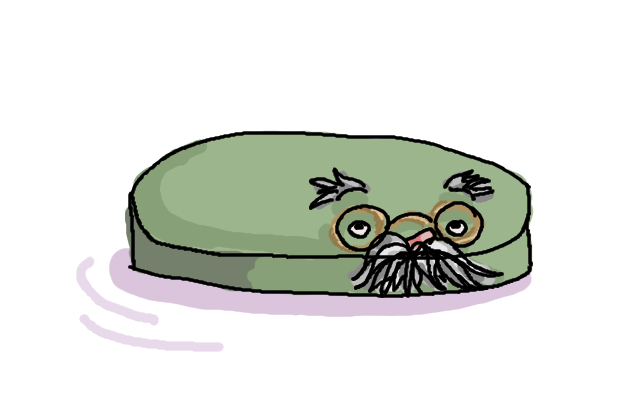
\includegraphics[width=0.9\linewidth]{Pictures/SP/norbert.png} 
\label{fig:norbert}
\end{wrapfigure}
Deswegen muss er so schnell wie möglich zurück zur Aufladestation.
Das Zimmer ist gefliest und Norbert kann von einer Fliese auf die andere fahren (das nennt er Schritt), aber nur nach vorne, nach hinten, nach links oder nach rechts, weil er sich nur um 90 Grad drehen kann. Ausserdem stehen im Zimmer Möbel herum, unter welchen Norbert nicht passt. Wie viele Schritte muss er bis zur Aufladestation fahren?

Norbert hat eine ziemlich gute mentale Karte vom Zimmer. Er weiss, dass das Zimmer 8 mal 6 Fliesen gross ist und einige grosse Schränke, Bücherregale und Sofas enthält. Er weiss genau, wo jedes Möbelstück steht.
\begin{figure}[H]
    \centering
    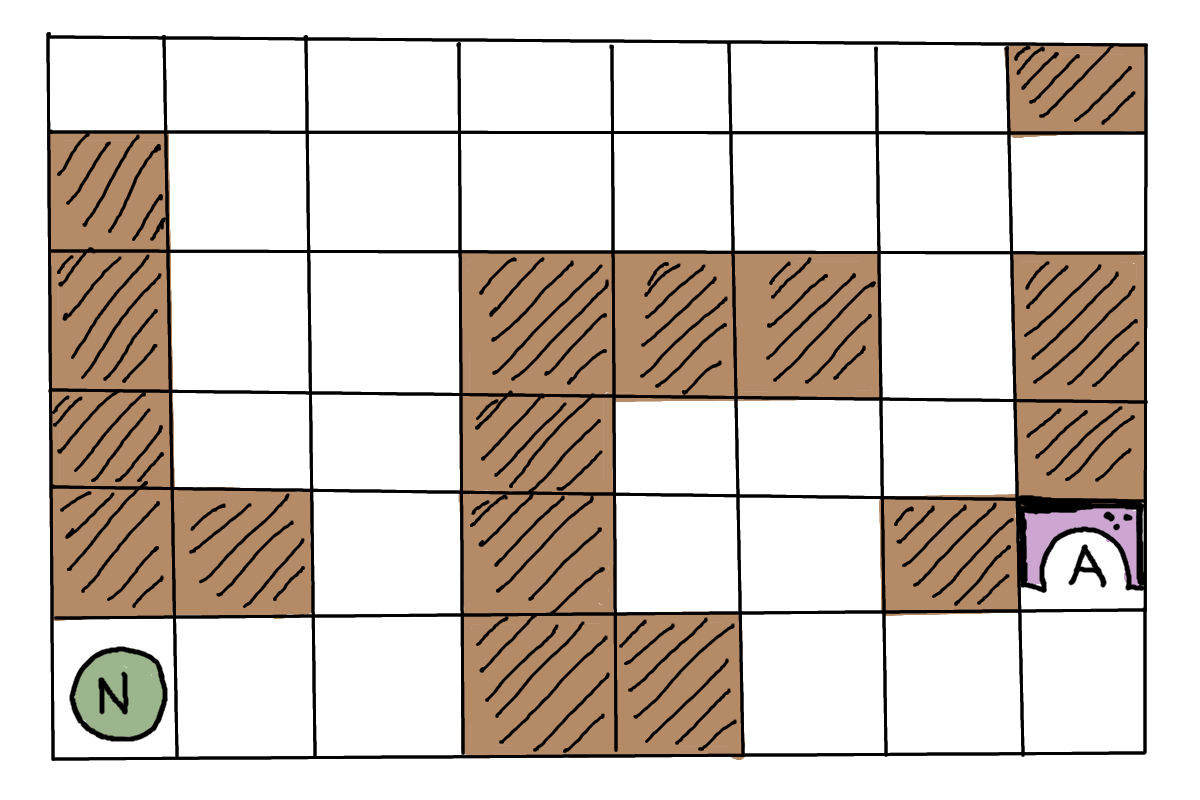
\includegraphics[width=\textwidth]{Pictures/SP/norbert_zimmer.png}
    \caption{Das Zimmer, wo sich Norbert befindet. In braun sind die Möbel markiert, unter welchen Norbert nicht passt. Norbert ist unten links, die Aufladestation ist unten rechts.}
    \label{fig:norbert_zimmer}
\end{figure}

\begin{aufgabe}\label{aufgabe_norbert}
\begin{enumerate}[(a)]
\item Modelliere das Problem von Norbert als Graph. Was sind die Knoten? Was sind die Kanten? Ist der Graph gerichtet? Wie modellierst du die Möbel?
\item Norbert hat nur noch Akku für 15 Schritte. Benutze den abgeänderten Breitensuchealgorithmus, um herauszufinden, ob er es noch schafft, die Aufladestation zu erreichen.
\item Wie viel Akku muss Norbert mindestens haben (gemessen in Schritte, die er noch machen kann), wenn er sicher sein will, dass er aus jeder Position im Zimmer die Aufladestation erreichen kann?
\item Schreibe den Graphen, den du aus Abbildung \ref{fig:norbert_zimmer} modelliert hast, in Python in der ''Liste der Nachbarn''-Darstellung.
\item Führe das Programm \texttt{length\_shortest\_path} aus, um die Länge des kürzesten Pfades zwischen Norbert und der Aufladestation zu bestimmen. Vergleiche das Ergebnis mit dem, was du in der Teilaufgabe (b) berechnet hast.
\end{enumerate}
\end{aufgabe}



\subsection{Der kürzeste Pfad}
Es ist sicher nützlich zu wissen, dass Bob in nur drei Klicks den Wikipedia-Artikel über den Zürcher Strassenbahnnetz erreichen kann, wenn der beim Breitensucheartikel startet; oder dass Alice über 3 Ecken jemanden kennt, der von einem Panda gebissen wurde; oder dass Norbert der Staubsauger-Roboter in 18 Schritten die Aufladestation erreichen kann. Aber wäre es nicht noch nützlicher zu wissen, welche Links Bob anklicken, oder welche Freunde und Freundesfreunde Alice kontaktieren, oder wo lang Norbert fahren müssen?

\subsubsection*{Norbert der Staubsauger-Roboter}
In einer Kontrollaufgabe haben wir Norbert den Staubsauger-Roboter kennengelernt. Der Boden des Zimmers, welches Norbert putzt, ist gefliest, und Norbert kann in einem ''Schritt'' von der Fliese, wo er ist, auf eine Fliese fahren, die sich vor ihm, hinter ihm, links von ihm oder rechts von ihm befindet. Aber es gibt Fliesen, auf welchen er nicht fahren kann, denn dort stehen Möbel (Schränke, Bücherregale, Sofas), unter welchen Norbert nicht passt. Norbert weiss genau, wo er sich befindet, wo die Aufladestation ist und wo all die Möbel stehen, die er umfahren muss.
\begin{figure}[H]
    \centering
    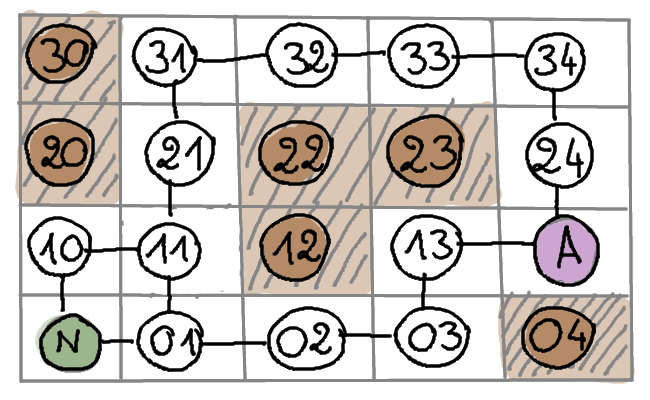
\includegraphics[width=0.6\textwidth]{Pictures/SP/norbert_klein_graph.png}
    \caption{Ein Zimmer für Norbert, schon als Graph modelliert. Die braunen isolierten Knoten stellen die Möbel dar.}
    \label{fig:norbert_klein_graph}
\end{figure}
Wir können das Zimmer als Graph modellieren, indem wir jeder Fliese einen Knoten zuordnen. Zwischen zwei Knoten gibt es eine Kante, wenn Norbert von der ersten entsprechenden Fliese auf die zweite in einem ''Schritt'' fahren kann.

Wir werden jetzt Norbert den Staubsauger-Roboter helfen, so schnell wie möglich seine Aufladestation zu erreichen. Wie auch für die Länge des kürzesten Pfades, gibt uns der Breitensuchealgorithmus alle benötigten Informationen, wir müssen sie nur speichern und richtig verwenden.

Nehmen wir an, wir führen jetzt die klassische Breitensuche aus. Wir fangen beim Startknoten \textbf{N} an und fügen dessen zwei Nachbarn \textbf{01} und \textbf{10} in die Warteschlange ein. Dann entfernen wir \textbf{01} aus der Warteschlange und fügen dessen Nachbarn hinzu: \textbf{02} und \textbf{11}. Dann entfernen wir \textbf{10}, welcher keine unbesuchten Nachbarn hat. Dann entfernen wir \textbf{02} und fügen \textbf{03} ein. Dann entfernen wir \textbf{11} und fügen \textbf{21} ein. Dann entfernen wir \textbf{03} und fügen \textbf{13} ein. Dann entfernen wir \textbf{21} und fügen \textbf{31} ein. Dann entfernen wir \textbf{13} und wir haben \textbf{A} schon gefunden. Die Knoten werden also in der folgenden Reihenfolge besucht.
\begin{lstlisting}[language=Python]
visited = ["N", "01", "10", "02", "11", "03", "21", "13", "31", "A"]
\end{lstlisting}
Aber wie können wir jetzt daraus den Pfad ausrechnen?


Die wichtige Beobachtung ist, dass wir \textbf{A} als Nachbar von \textbf{13} gefunden haben. Wir sagen dazu, dass \textbf{13} der \textbf{Elternknoten} von \textbf{A} ist. Das bedeutet, dass der kürzeste Pfad von \textbf{N} nach \textbf{A} über \textbf{13} verläuft.
\begin{figure}[H]
    \centering
    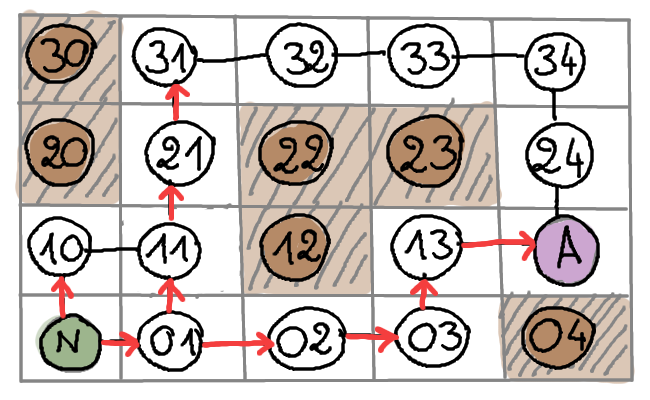
\includegraphics[width=0.6\textwidth]{Pictures/SP/norbert_klein_graph_arrows.png}
    \caption{Wir haben mit roten Pfeilen die Kanten markiert, welche wir bei der Breitensuche verwendet hatten. Um den kürzesten Pfad von \textbf{N} nach \textbf{A} zu finden, müssen wir nur die Pfeile von \textbf{A} nach \textbf{N} zurückverfolgen.}
    \label{fig:norbert_klein_graph_arrows}
\end{figure}
Wenn es einen kürzeren Pfad über einen anderen Knoten gegeben hätte, hätten wir \textbf{A} früher gefunden als Nachbar von einem anderen Knoten als \textbf{13}. Also muss \textbf{13} auf dem kürzesten Pfad liegen. Wir haben nun das Problem reduziert: Wir müssen nur noch den kürzesten Pfad zwischen \textbf{N} und \textbf{13} finden.

Wir gehen analog vor und fragen uns, woher wir \textbf{13} erreicht haben, das heisst wir suchen dessen Elternknoten. Den Knoten \textbf{13} haben wir als Nachbar von \textbf{03} gefunden. Dann muss \textbf{03} auch auf dem kürzesten Pfad liegen. Diese Kette lässt sich weiter führen: Den Knoten \textbf{03} haben wir von \textbf{02} aus gefunden, und \textbf{02} von \textbf{01} aus, und \textbf{01} von \textbf{N} aus. Der kürzeste Pfad ist somit:
\begin{lstlisting}
N - 01 - 02 - 03 - 13 - A.
\end{lstlisting}

Um den kürzesten Pfad aufzulisten, haben wir die roten Pfeilen aus Abbildung \ref{fig:norbert_klein_graph_arrows} zurückverfolgt, von \textbf{A} zurück nach \textbf{N}, in der umgekehrten Reihenfolge, in der die Breitensuche sie gefunden hatte. Diesen Verfahren nennt man \textbf{Backtracking}.

Aus einem Knoten können mehrere ''rote Pfeile'' ausgehen (weil ein Knoten mehrere Nachbarn haben kann, die wegen ihm in die Warteschlange eingefügt werden), aber maximal ein Pfeil kann darauf zeigen (weil wir Knoten, die wir schon gesehen haben, kein zweites Mal in die Warteschlange einfügen). Alle ''rote Pfeile'', wenn wir sie in die andere Richtung verfolgen, führen nach \textbf{N}, und zwar über den kürzesten Pfad.

\begin{aufgabe}\label{aufgabe_find_shortest_path}
Betrachte folgenden Graphen. 
\begin{figure}[H]
    \centering
    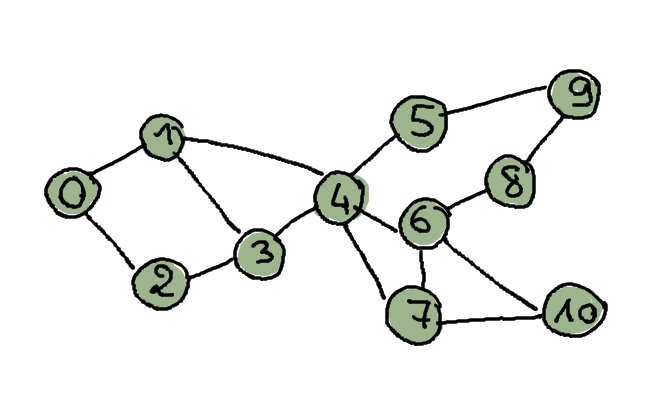
\includegraphics[width=0.6\textwidth]{Pictures/SP/shortest_path_graph.png}
\end{figure}
\begin{enumerate}[(a)]
    \item Finde den küzesten Pfad zwischen \textbf{0} und \textbf{9}. Benutze einen Breitensuche-ähnlichen Verfahren.
    \item Was würdest du machen, wenn du jetzt den kürzesten Pfad zwischen \textbf{0} und \textbf{10} finden müsstest? Kannst du etwas aus der vorherigen Teilaufgabe wiederverwenden?
    \item Wie würdest du den kürzesten Pfad zwischen \textbf{6} und \textbf{0} finden? Kannst du etwas aus den vorherigen Teilaufgaben wiederverwenden?
    \item Und wenn du den kürzesten Pfad zwischen \textbf{9} und \textbf{1} finden musst?
\end{enumerate}{}
\end{aufgabe}

\begin{aufgabe}\label{aufgabe_shortest_path_alg}
Überlege wie du den Breitensuchealgorithmus verändern musst, um den kürzesten Pfad zwischen zwei Knoten zu finden. Du kannst deine Erkenntnisse aus Aufgabe \ref{aufgabe_find_shortest_path} benutzen.

Welche zusätzliche Informationen musst du speichern? Wo würdest du es machen?
Wie verwendest du diese zusätzliche Informationen, um den Pfad zu finden?

Schreibe deinen Algorithmus möglichst genau auf.
\end{aufgabe}



\subsubsection*{Der kürzeste Pfad in Python}
Wir werden jetzt zusammen eine mögliche Lösung zur Aufgabe \ref{aufgabe_shortest_path_alg} in Python implementieren. Die zwei wichtigen Unterschiede zum ersten Breitensucheprogramm haben mit den roten Pfeilen aus Abbildung \ref{fig:norbert_klein_graph_arrows} zu tun:
\begin{enumerate}
    \item Wie wir die ''rote Pfeile'' speichern
    \item Wie wir die ''rote Pfeile'' zurückverfolgen
\end{enumerate}

Zuerst werden wir das erste Breitensucheprogramm so verändern, dass wir uns für jeden besuchten Knoten merken, woher wir diesen Knoten gefunden haben. Das Programm erwartet einen Graphen und einen Startknoten und gibt für jeden erreichbaren Knoten aus, woher wir diesen Knoten gefunden haben.

\begin{lstlisting}[language=Python, caption={Programm, welches die ''rote Pfeile'' ausgehend von einem Startknoten berechnet und ausgibt. Die einzigen zwei Zeilen, die sich verändert haben, sind 3 und 10.}, label={bfs_with_parent}]
def bfs_with_parent(graph, initial):
    queue = [initial]
    visited = {initial:None}
    while queue:
        node = queue.pop(0)
        neighbours = graph[node]
        for neighbour in neighbours:
            if neighbour not in visited:
                queue.append(neighbour)
                visited[neighbour] = node
    return visited
\end{lstlisting}
Verändert haben sich die Zeilen 3 und 10. Beobachte, dass wir für die besuchten Knoten keinen Vektor mehr brauchen, sondern ein assoziatives Datenfeld, welches jedem Knoten seinen Elternknoten (das nicht spitze Ende vom ''roten Pfeil'') zuordnet. In der dritten Zeile ordnen wir dem Startknoten den speziellen Wert \texttt{None} zu, um zu signalisieren, dass er keinen Elternknoten hat. In der zehnten Zeile ordnen wir jedem neuen unbesuchten Nachbarn seinen Elternknoten zu.

Führe das Programm auf den Graphen aus der Aufgabe \ref{aufgabe_find_shortest_path} aus. Kannst du alle ''rote Pfeile'' in der Ausgabe wieder finden?
\begin{lstlisting}[language=Python]
numbers = {0: [1, 2],
        1: [0, 3, 4],
        2: [0, 3],
        3: [1, 2, 4],
        4: [1, 3, 5, 6, 7],
        5: [4, 9],
        6: [4, 7, 8, 10],
        7: [4, 6, 10],
        8: [6, 9],
        9: [5, 8],
        10:[6, 7]}

print(bfs_with_parent(numbers, 0))
{0: None, 1: 0, 2: 0, 3: 1, 4: 1, 5: 4, 6: 4, 7: 4, 8: 6, 9: 5, 10: 6}
\end{lstlisting}

Um den kürzesten Pfad zu finden, reicht es nicht, die ''roten Pfeilen'' auszugeben. Wir müssen sie auch \textbf{zurückverfolgen}.
Jetzt schreiben wir ein Programm, \texttt{backtracking}, welches genau das macht. Das Programm erwartet ein assoziatives Datenfeld, welches jedem Knoten seinen Elternknoten zuordnet (genau wie die Ausgabe von \texttt{bfs\_with\_parent}), und einen Zielknoten, und gibt den kürzesten Pfad zurück.

\begin{lstlisting}[language=Python, caption={Programm, welches ''rote Pfeile'' zurückverfolgt}, label={backtracking}]
def backtracking(parents, goal):
    reversed_path = []
    node = goal
    while node != None:
        reversed_path.append(node)
        node = parents[node]
    return list(reversed(reversed_path))
\end{lstlisting}
Das Programm fängt beim Zielknoten an und schlägt im assoziativen Datenfeld nach, woher dieser Knoten gefunden wurde. Er schlägt den Elternknoten im assoziativen Datenfeld und dessen Elternknoten und dessen Elternknoten, und es macht so weiter, bis es einen Knoten findet, der keinen Elternknoten hat. Dieser Knoten muss der Startknoten der Breitensuche gewesen sein. Mit all diesen Knoten füllt es nach und nach einen Vektor.

Beobachte, dass wir den Pfad in der letzten Zeile umdrehen müssen, sonst kriegen wir den kürzesten Pfad vom Ziel- zum Startknoten.

\begin{aufgabe}\label{aufgabe_shortest_path}
Schreibe ein Programm in Python, welches, gegeben ein Graph, ein Start- und ein Zielknoten, den kürzesten Pfad zwischen Start- und Zielknoten ausgibt. Du kannst dafür \texttt{bfs\_with\_parent} und \texttt{backtracking} verwenden.
\end{aufgabe}

\begin{framed}
\paragraph{\textcolor{blue-violet}{Was haben wir gelernt:}}
Um den \textbf{kürzesten Pfad} zwischen Start- und Zielknoten in einem Graphen zu finden, können wir eine abgeänderte Version vom Breitensuchealgorithmus verwenden. Wie in der normalen Breitensuche, verwenden wir eine Warteschlange, um die zu besuchenden Knoten zu speichern. Aber in dieser Version enthält die Warteschlange nicht nur die zu besuchende Knoten, sondern auch deren \textbf{Elternknoten}, das heisst den Knoten, wegen dem sie in die Warteschlange gelandet sind. Wir ordnen also jedem Knoten \textbf{höchstens einen} Knoten zu, als dessen Nachbar sie zur Warteschlange hinzugefügt worden sind.

Der Startknoten und jene Knoten, die vom Startknoten weiter entfernt sind als der Zielknoten, haben keinen Elternknoten.

Um den kürzesten Pfad zu finden, müssen wir die Elternknoten vom Zielknoten aus zurückverfolgen. Diesen Prozess nennt man \textbf{Backtracking}.
\end{framed}

\subsubsection*{Ein Spaziergang im All}
\begin{figure}[H]
    \centering
    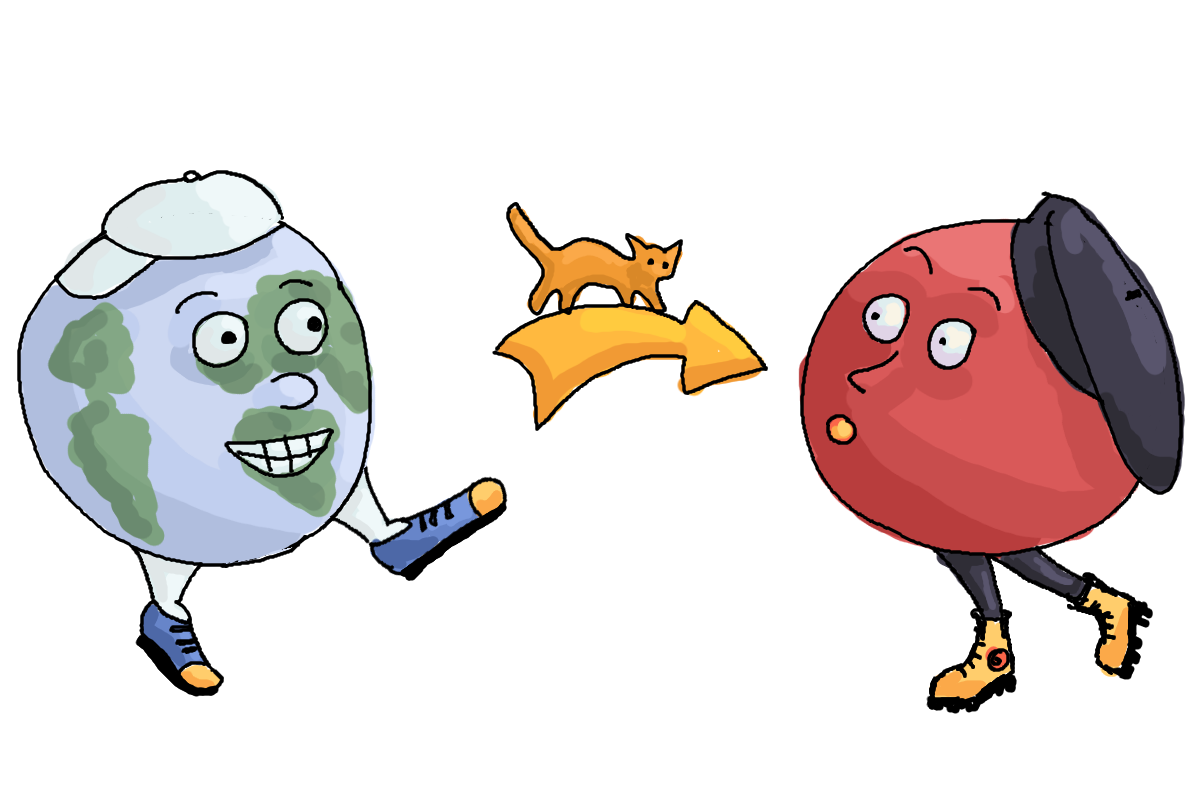
\includegraphics[width=\textwidth]{Pictures/SP/erde_mars.png}
\end{figure}
Wie weit ist es von der Erde bis zum Mars? Es kommt darauf an, wie man es misst! Wir behaupten, dass der Abstand kleiner oder gleich 12 sein muss. Und wie weit ist es von der Hand bis zum Fuss?
\begin{lstlisting}
HAND - FAND - FANS - FASS - FUSS
\end{lstlisting}
Der Sinn vom Spiel ist es eine möglichst kurze Folge von Wörter zu finden, die das Start- mit dem Zielwort verbindet, wobei alle Wörter genau 4 Buchstaben haben und zwei Wörter dürfen genau dann daneben stehen, wenn sie sich genau um einen Buchstaben unterscheiden.


\begin{aufgabe}
\begin{enumerate}[(a)]\label{aufgabe_erde_mars_graph}
    \item Formuliere das Spiel als Graph. Was sind die Knoten? Wann gibt es eine Kante zwischen zwei Knoten? Ist der Graph gerichtet oder ungerichtet?
    \item Zeichne den Graphen, der folgende Wörter modelliert:
\begin{lstlisting}
BANK, ZINS, ZANK, SINN, SAND, ZINK, SANK, ZINN
\end{lstlisting}
    \item Gibt es einen Pfad zwischen \textbf{\texttt{BANK}} und \textbf{\texttt{ZINS}}, welcher nur aus den aufgelisteten Wörter besteht?
    \item Wenn du das Wort \textbf{\texttt{ZINK}} entfenst, kannst du zwei Wörter hinzufügen, so dass \textbf{\texttt{BANK}} und \textbf{\texttt{ZINS}} immer noch verbunden sind?
\end{enumerate}

\end{aufgabe}

\begin{figure}[H]
    \centering
    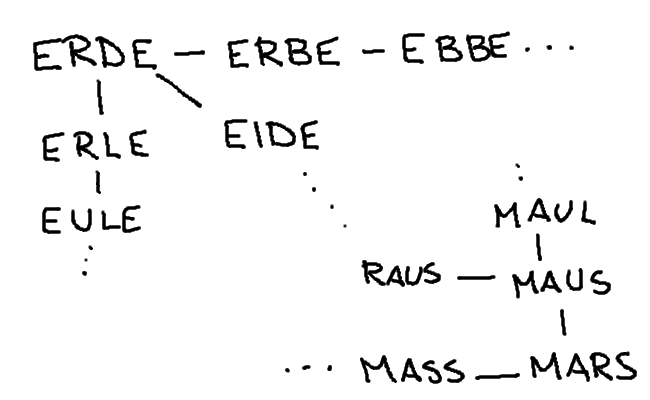
\includegraphics[width=\textwidth]{Pictures/SP/erde_mars_first_graph.png}
\end{figure}

\begin{aufgabe}\label{aufgabe_erde_mars_neighbours}
\begin{enumerate}[(a)]
    \item Schreibe den Graphen über den folgenden Wörter in der Liste der Nachbarn Darstellung.
    \begin{lstlisting}
    ERDE, EIDE, EINE, EINS, ZINS, ZINK, ZANK, ZACK, PACK, PARK, MARK, MARS,
    MAUS, HAUS, HASS, BASS, PARD, BAND, SAND, SACK, BANK, SANK, SINN, ZNINN,
    ZICK, PINS, EILT, EILE, EULE, ERLE, ENTE, ENDE
    \end{lstlisting}
    \item Rufe das Programm aus der Aufgabe \ref{aufgabe_shortest_path} auf und finde den kürzesten Pfad zwischen Erde und Mars heraus.
    \item ** Du hast bestimmt bemerkt, wie mühsam und fehleranfällig es ist, solche Graphen selber zu konstruieren und zu erweitern. Dabei ist die Idee dahinter ziemlich einfach: Nachbarwörter unterscheiden sich um einen Buchstaben. Verwende deine Kenntnisse in der Stringmanipulation und Stringkomposition, um ein Programm zu schreiben, das eine Menge von Wörter und ein Wort erwartet und alle Nachbarwörter des Wortes ausgibt, die in der Menge der Referenzwörter enthalten sind.
    \item * Schreibe das Programm aus der Aufgabe \ref{aufgabe_shortest_path} so um, dass es den Graphen nicht als Liste der Nachbarn erwartet, sondern als Liste aller Knoten, und verwende dein Programm aus der vorherigen Teilaufgabe, um die Nachbarn zu berechnen.
\end{enumerate}
\end{aufgabe}
Jetzt können wir noch mehr Wörter hinzufügen und herausfinden, was weiter von der Erde ist: der Mond oder der Mars.

\subsubsection*{\textcolor{blue-violet}{Teste dich selber}}
\begin{aufgabe}\label{pfad_kontrollfragen}
Beantworte folgende Fragen.
\begin{enumerate}[(a)]
\item Was hat die Breitensuche mit dem kürzesten Pfad zwischen zwei Knoten zu tun?
\item Welche zusätzliche Informationen muss man während der Ausführung des Breitensuchealgorithmus speichern, wenn man den kürzesten Pfad zwischen Start- und Zielknoten bestimmen möchte?
\item Was ist Backtracking? Wozu braucht man das?
\item Gregory behauptet: ''Wenn man vom Startknoten ausgehend alle Elternknoten mit dem abgeänderten Breitensuchealgorithmus findet, kann man den kürzesten Pfad zwischen dem Startknoten und allen anderen Knoten bestimmen, ohne die Breitensuche ein zweites Mal ausführen zu müssen''. Hat er recht? Begründe deine Antwort.
\item Hannah behauptet: ''Wenn man von einem Knoten ausgehend alle Elternknoten einmal berechnet hat, kann man dann den kürzesten Pfad zwischen zwei beliebigen Knoten im Graphen bestimmen, ohne die Breitensuche nochmal ausführen zu müssen.'' Hat sie recht? Begründe deine Antwort.
\end{enumerate}
\end{aufgabe}

\begin{aufgabe}\label{wikipedia_kontrollaufgabe}
Betrachte folgenden Graphen, welcher die Verlinkung von 11 Wikipediaartikeln darstellt.
\begin{figure}[H]
    \centering
    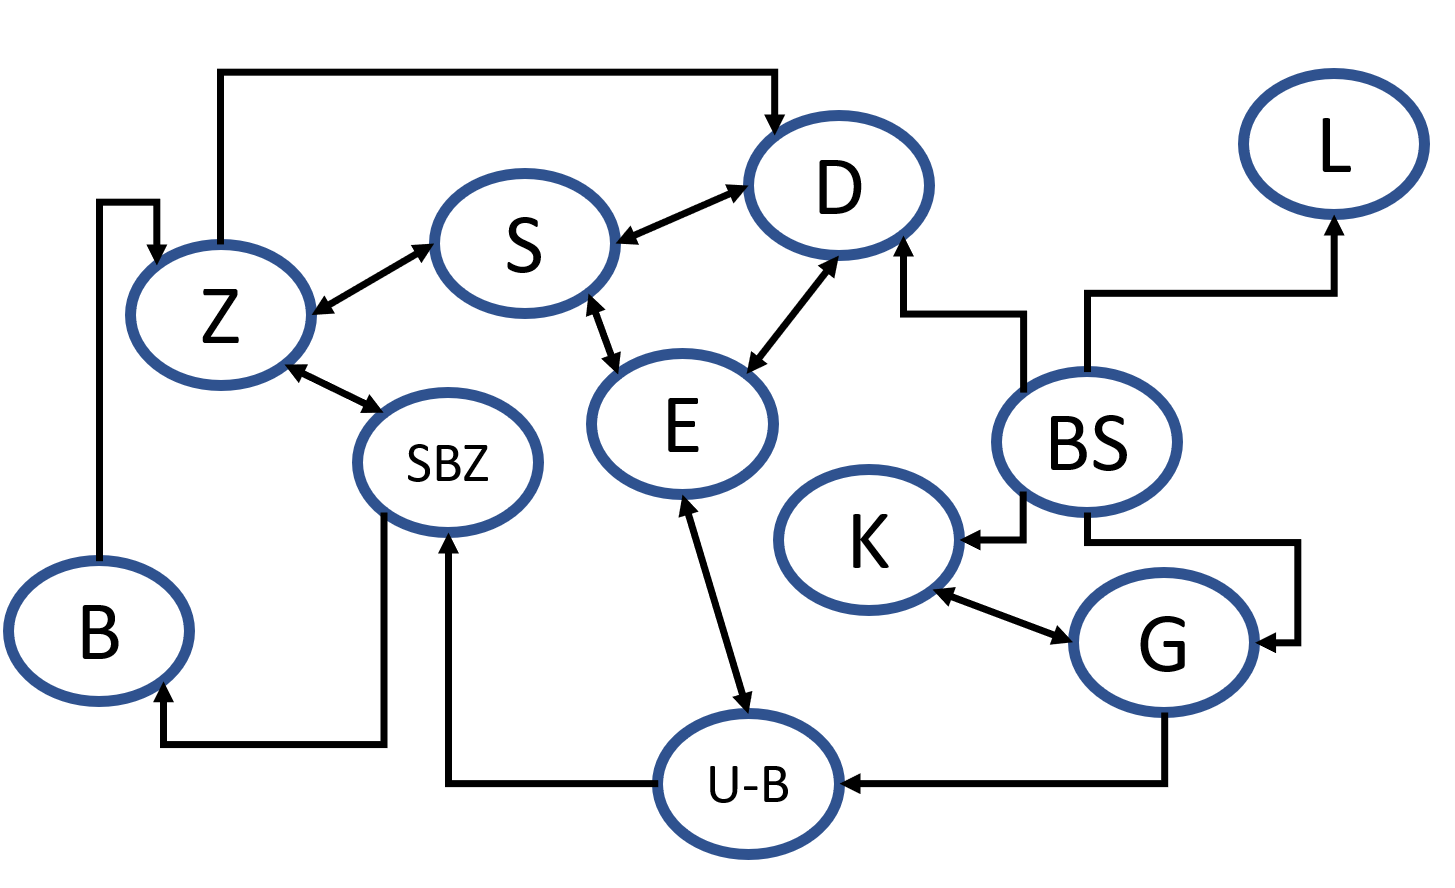
\includegraphics[width=0.7\textwidth]{Pictures/Wikipedia.PNG} 
    \caption{Die Verlinkung von Wikipediaartikeln als Graph.}
\end{figure}
\begin{enumerate}[(a)]
\item Benutze die Breitensuche, um den kürzesten Pfad zwischen \textbf{B} und \textbf{U-B} zu finden.
\item Benutze die Breitensuche, um den kürzesten Pfad zwischen \textbf{Z} und \textbf{L} zu finden.
\item Hannah behauptet: ''Wenn du \textbf{BS} als Zielknoten angibst, dann hat der Gegner keine Chance!''. Hat sie recht? Wieso?
\item Gregory behauptet: ''Um den kürzesten Pfad zwischen \textbf{B} und \textbf{D} zu finden, muss ich einfach den kürzesten Pfad zwischen \textbf{D} und \textbf{B} umdrehen.'' Stimmt das?
\item Benutze die Breitensuche, um die kürzeste Pfade zwischen \textbf{B} und \textbf{S}, zwischen \textbf{B} und \textbf{D} und zwischen \textbf{B} und \textbf{E} zu finden. Ist es einfacher, als die kürzesten Pfade zwischen \textbf{Z} und \textbf{D}, zwischen \textbf{U-B} und \textbf{D} und zwischen \textbf{SBZ} und \textbf{D} zu finden? Wieso?
\end{enumerate}
\end{aufgabe}

\paragraph{Schlangenspiel}
Alice und Bob sind zufällig in den Kinderabteil eines Zuges gelandet. Auf dem Tisch ist ein Schlangenspiel gezeichnet.
\begin{figure}[H]
    \centering
    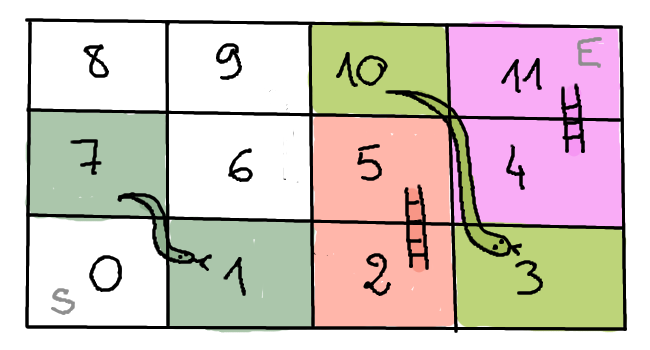
\includegraphics[width=\textwidth]{Pictures/SP/schlangen_spiel.png}
\end{figure}
Sie haben zwar keinen Würfel, aber sie verwenden zwei Münzen, um einen Würfel mit 4 Seiten zu simulieren (zum Beispiel, \texttt{(KOPF, ZAHL)} entspricht einer 1, \texttt{(ZAHL, KOPF)} einer 2, \texttt{(ZAHL, ZAHL)} einer 3 und \texttt{(KOPF, KOPF)} einer 4).
Bob will um jeden Preis gewinnen. Er hat schon herausgefunden, wie er die Resultate seiner Münzenwürfe steuert. Aber er weiss nicht, welche Zahlen rauskommen müssen, damit er mit möglichst wenig Münzenwürfe das Ziel erreicht.

\begin{aufgabe}\label{aufgabe_schlangenspiel}
\begin{enumerate}[(a)]
    \item Formalisiere das Schlangenspiel als Graph. Was sind die Knoten? Wann gibt es eine Kante zwischen zwei Knoten? Ist der Graph gerichtet oder ungerichtet?
    \item Schreibe das kleinere Spielfeld in der ''Liste der Nachbarn''-Darstellung.
    \item Was muss Bob würfeln, um zu gewinnen? Führe das Programm aus der Aufgabe \ref{aufgabe_shortest_path} aus.
    \item Schreibe das Programm aus der Aufgabe \ref{aufgabe_shortest_path} so um, dass es die Zahlen ausgibt (1, 2, 3, 4), die Bob erzielen muss.
    \item ** Überlege, was du brauchst, um die Nachbarn zu berechnen. Schreibe ein Programm, welches alle Nachbarn von einem Knoten ausgibt.
    \item * Kombiniere deine Programme aus den vorherigen Teilaufgaben und helfe Bob das Schlangenspiel auf dem grossen Spielfeld zu gewinnen. Was muss er würfeln?
    \begin{figure}[H]
    \centering
    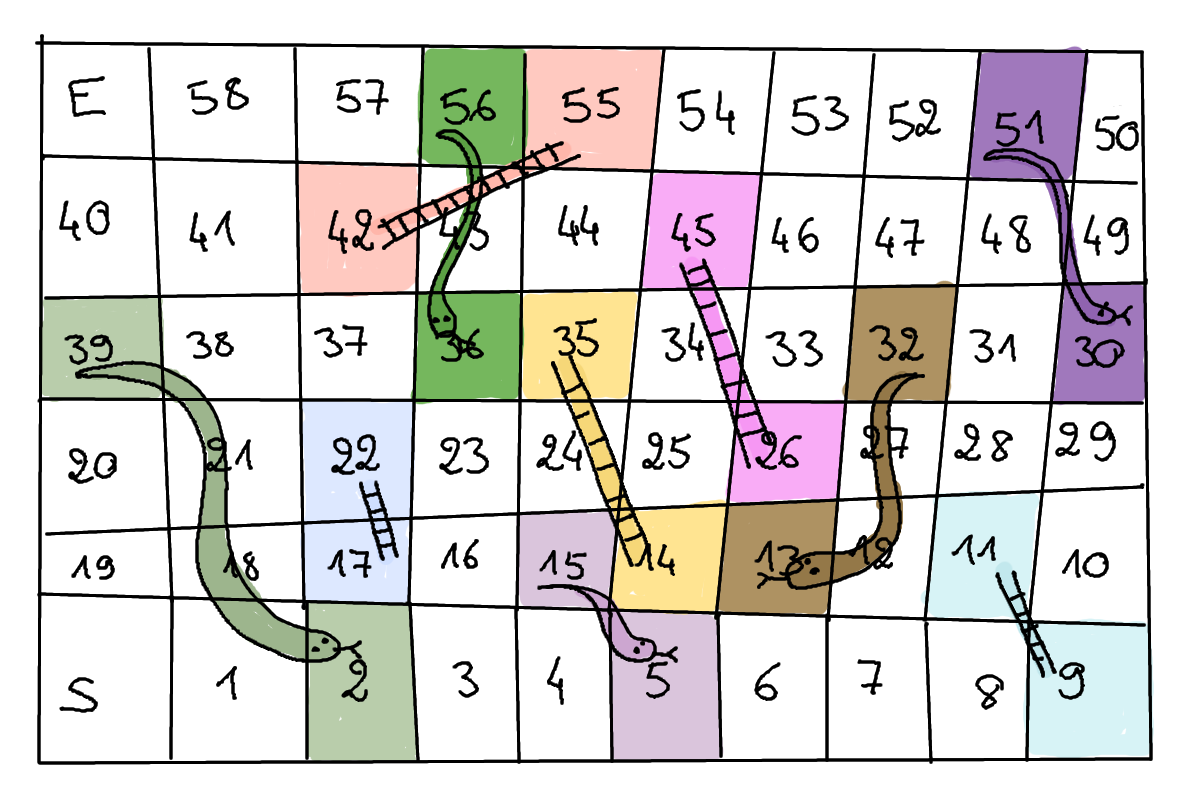
\includegraphics[width=\textwidth]{Pictures/SP/snakes_ladders_big.png}
\end{figure}
\end{enumerate}
\end{aufgabe}

\newpage

\section{Zusammenfassung}
Du hast mit der Breitensuche deinen ersten Algorithmus für Graphen kennengelernt. Der Algorithmus nimmt als Eingabe einen Graphen und einen Startknoten in diesem Graphen und durchläuft dann alle Knoten in der gleichen Zusammenhangskompnente wie der Startknoten, geordnet nach aufsteigendem Abstand vom Startknoten. Man kann den Algorithmus auch so abändern, dass man als Eingabe zusätzlich einen gesuchten Zielknoten gibt und die Suche abbricht, sobald dieser gefunden wurde.

Du hast gelernt, dass du den Algorithmus leicht abändern kannst, um den Abstand zwischen zwei Knoten zu ermitteln. Dafür musst du dir für jeden besuchten Knoten merken, wie weit er vom Startknoten entfernt war.

Wenn du dir, anstatt vom Abstand zum Startknoten, für jeden Knoten merkst, von welchem Elternknoten aus er besucht wurde, kriegst du genug Informationen, um daraus den kürzesten Pfad zwischen dem Startknoten und allen anderen Knoten berechnen zu können. Das machst du dann mit Backtracking, indem du alle Elternknoten vom Zielknoten bis zum Startknoten in umgekehrter Reihenfolge aneinander reihst. Wenn sich der Startknoten nicht ändert, es genügt das Backtracking mit dem neuen Zielknoten auszuführen.

Ausserdem hast du gesehen, wie sich viele unteschiedliche Probleme als Graphprobleme modellieren und lösen lassen. Zum Beispiel, hast du gesehen, dass Menschen, Haltestellen, Wikipediaartikel, Fliesen, Wörter und Spielkästchen als Knoten dienen können, und dass ein Staubsauger-Roboter, der zu seiner Aufladestation muss, sich im Grunde genommen nicht von einem Mädchen unterscheidet, welches unter ihren Bekannten eine von einem Panda gebissene Person sucht, oder von einem Jungen, der mit zwei gezinkten Münzen ein Schlangenspiel gewinnen will.
\newpage

\nocite{*}
\bibliographystyle{plain}
\bibliography{refs}
\newpage

\section{Beispiellösungen}
\paragraph{ Aufgabe \ref{newinitial}:} Wenn wir bei der Station ''Bellvue'' starten ist die Reihenfolge: $$ \text{\bf{B,KH,HP,KS,N,E/U,P,C,HB,HE}}$$

\paragraph{Aufgabe \ref{directed}:} Wir betrachten jetzt den folgenden Graphen:\\
\begin{figure}[H]
    \centering
    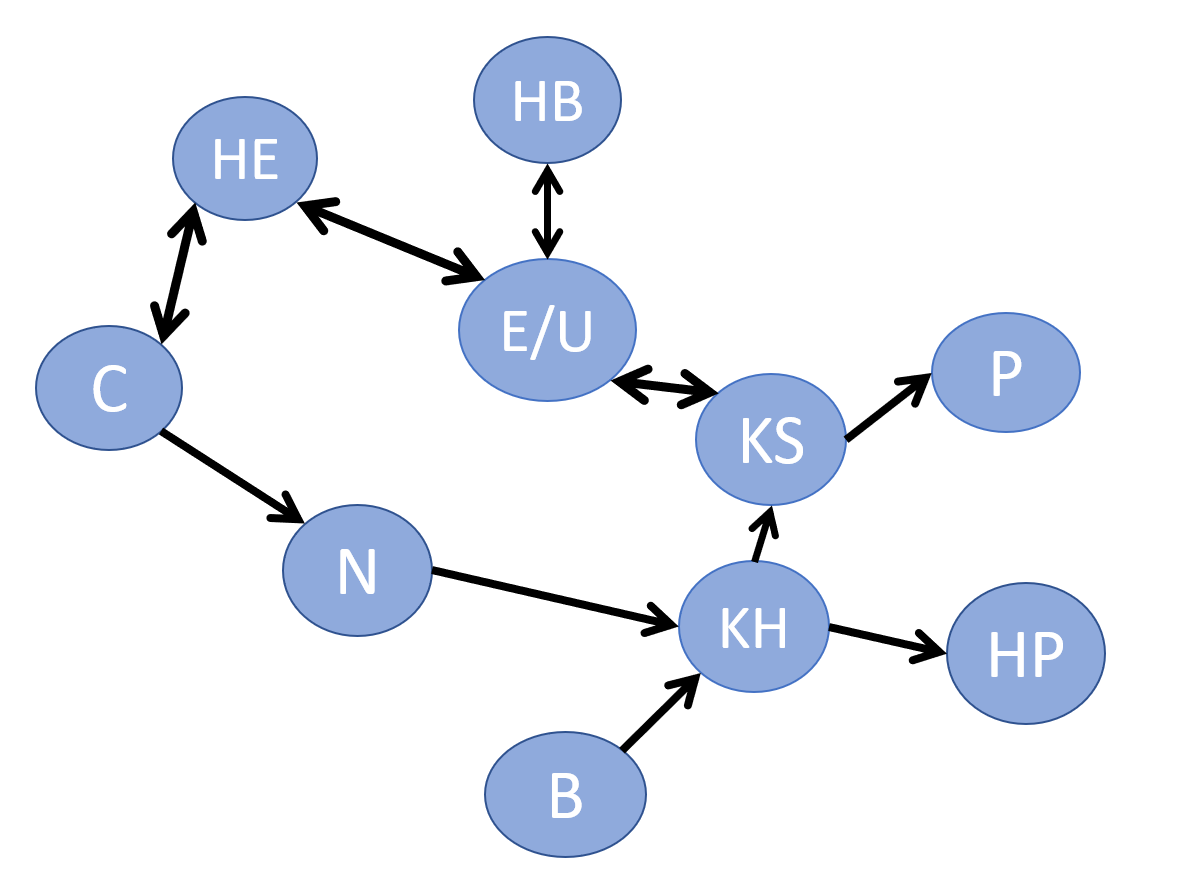
\includegraphics[scale=0.3]{Pictures/directedTram.PNG} 
    \caption{Der gerichtete Graph.}
    \label{fig:my_label}
\end{figure}
Die Reihenfolge in welcher die Breitensuche die Knoten besucht ist:
$$ \text{\bf{B,KH,HP,KS,E/U,P,HB,HE,C,N}}$$

\paragraph{Aufgabe \ref{Wikipedia}}: Wir beginnen die Breitensuche beim Wikipedia-Artikel über die Breitensuche; also bei dem Knoten {\bf{BS}}. Die Reihenfolge ist dann
$$ \text{\bf{BS,D,G,K,L,E,S,U-B,Z,SBZ}}.$$
Bob kann den gewünschten Artikel also finden und wir könen die Breitensuche abbrechen bevor wir den Knoten {\bf{B}} besucht haben.

\paragraph{Aufgabe \ref{ProgFragen}:} Die Liste ''queue'' enthält genau unsere Warteliste, in ''visited'' fügen wir Schritt für Schritt die besuchten Knoten hinzu, so dass wir am Ende mit ''return visited'' die Knoten in der gewünschten Reihenfolge zurückgeben können.

\begin{figure}[H]
    \centering
    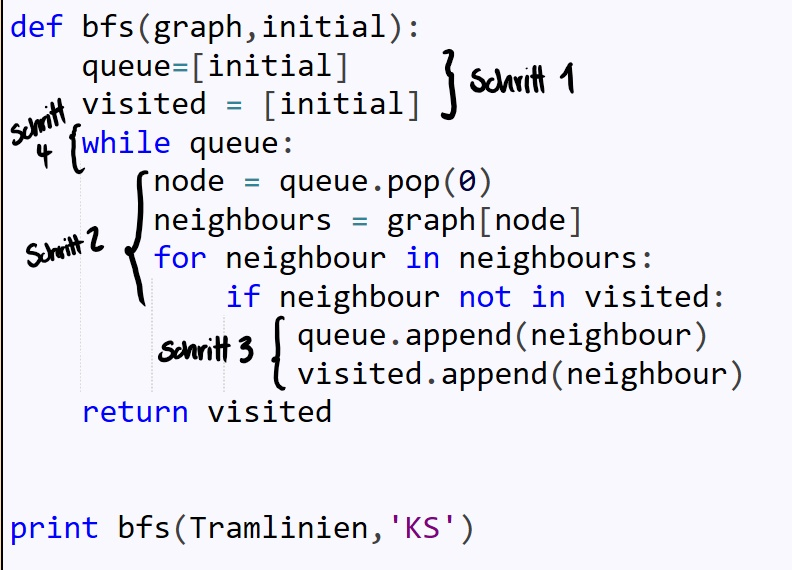
\includegraphics[scale=0.3]{Pictures/Loesung24.jpg}
    \caption{Die 4 Schritte des Algorithmus im Programm}
    \label{fig:ProgLoes}
\end{figure}

\paragraph{Aufgabe \ref{WikiProgAufg}:} Wir implementieren den Graphen der Wikipedia-Artikel in der ''Liste der Nachbarn''-Darstellung und passen das Programm an (Abbildung \ref{fig:my_Prog2Loes}). Falls der Start- und der Zielknoten gleich sind können wir die Suche sofort abbrechen. Ansonsten überprüfen wir jeweils nachdem wir einen Nachabrn als besucht markiert haben, ob dieser der gesuchte Knoten ist. Fall ja können wir die for-Schleife mit break beenden. Damit auch die while-Schleife endet leeren wir noch die Warteliste.

\begin{figure}[H]
    \centering
    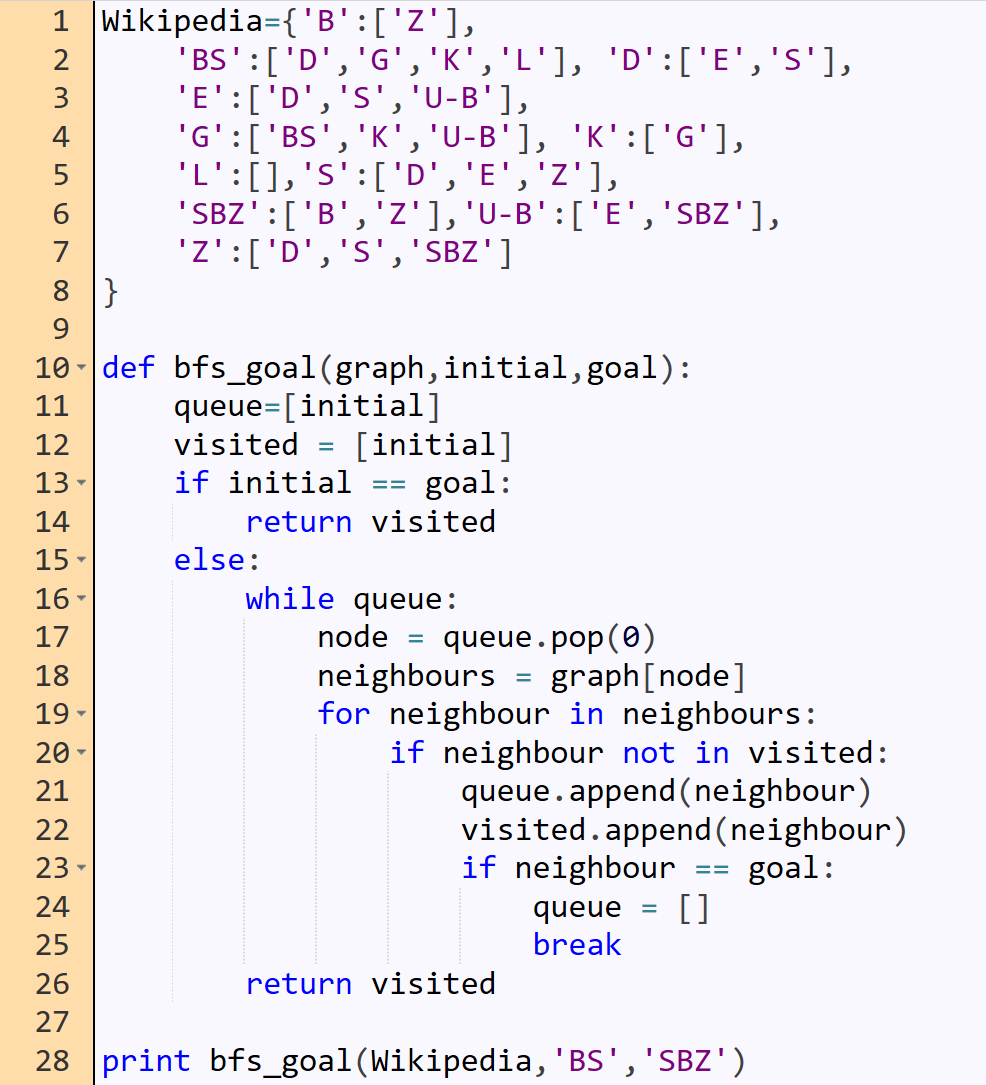
\includegraphics[scale=0.6]{Pictures/WikiProgLoes.PNG}
    \caption{Das Programm mit Zielknoten als Input und einer Abbruchsbedingung}
    \label{fig:my_Prog2Loes}
\end{figure}

\paragraph{Lernaufgabe} 
\begin{enumerate}
    \item Als Knoten nehmen wir alle Menschen. Wir verbinden je zwei Knoten wenn einer ein direkter Nachkomme vom anderen ist. Der Graph stellt also einfach einen Stammbaum dar.
    \item Sie können ''print bfs\_goal (Familien,'Alice','Bob')'' aufrufen. Falls bei der Ausgabe an letzter Stelle 'Bob' steht so haben sie eine gemeinsame Ur-ur-ur-ur-Grossmutter. Wenn die Breitensuche 'Bob' nicht findet, so sind Alice und Bob nicht so nahe verwandt.
    \item der gleichen Zusammenhangskomponente.
    \item Das angepasste Programm:
    \begin{figure}[H]
        \centering
        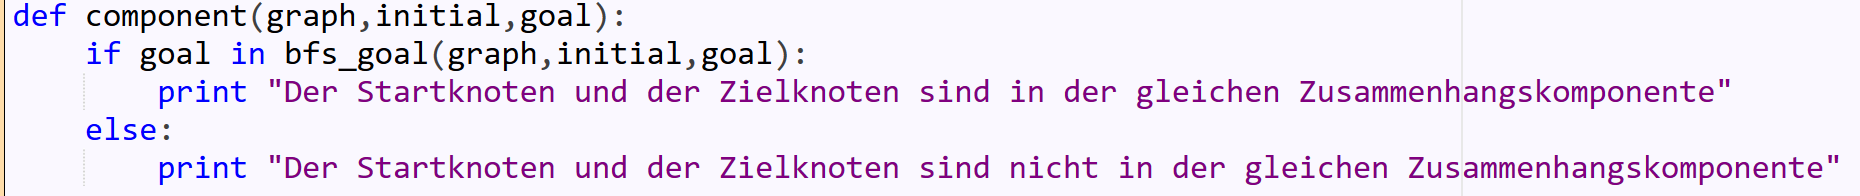
\includegraphics[scale=0.4]{Pictures/components.PNG}
        \caption{Wir rufen bfs\_goal auf und prüfen ob es den Zielknoten finden konnte.}
        \label{fig:my_components}
    \end{figure}
\end{enumerate}

\paragraph{Kontrollfragen}
\begin{enumerate}
    \item -
    \item - 
    \item Die Aussage von David ist falsch. Wir prüfen immer ob wir einen Knoten bereits besucht haben, bevor wir ihn auf die Warteliste setzen.
    \item Fred's Aussage stimmt nur für ungerichtete Graphen. In einem gerichteten Graphen kann es sein, dass man einen Knoten nicht findet, obwohl er sich in der gleichen Zusammenhangskomponente wie der Startknoten befindet.
    \item Gregory's Aussage ist richtig, er kann den Knoten ganz links als Startknoten nehmen in Abbildung \ref{fig:Gregory}.
    \begin{figure}[H]
        \centering
        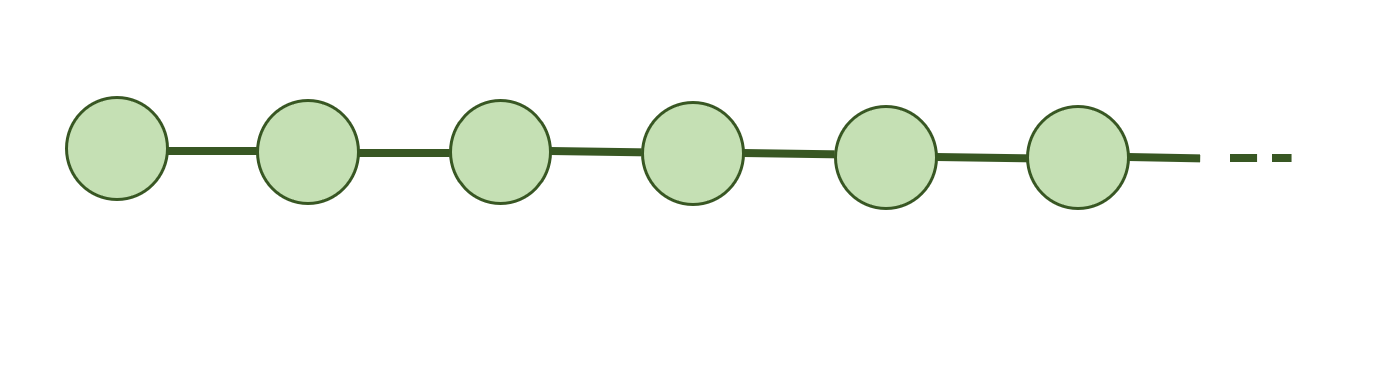
\includegraphics[width=\textwidth]{Pictures/Kontrollfragen.PNG}
        \caption{Gregory's Graph}
        \label{fig:Gregory}
    \end{figure}
\end{enumerate}

\paragraph{Aufgabe \ref{aufgabe_abstand_ex}}
Der Abstand zwischen \textbf{A} und \textbf{F} ist \(3\). Zwischen diesen Knoten gibt es die Pfade \textbf{ABEF}, \textbf{ACBEF} und \textbf{ACDEF}; der kürzeste Pfad hat Länge \(3\).
\begin{figure}[H]
    \centering
    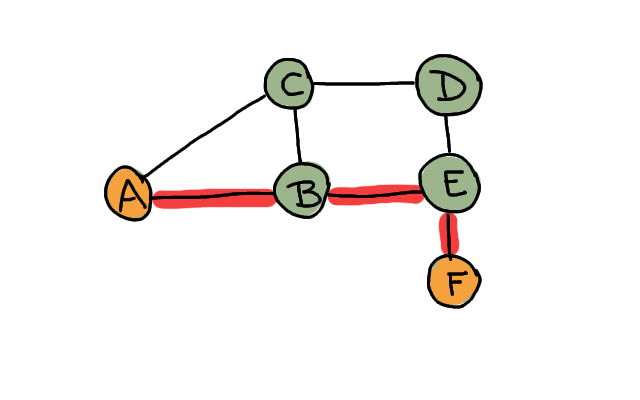
\includegraphics[width=0.5\textwidth]{Pictures/SP/abstand_ex-l1.png}
\end{figure}
Der Abstand zwischen \textbf{C} und \textbf{E} ist \(2\). Zwischen diesen Knoten gibt es die Pfade \textbf{CBE} und \textbf{CDE}. Beide haben Länge \(2\).
\begin{figure}[H]
    \centering
    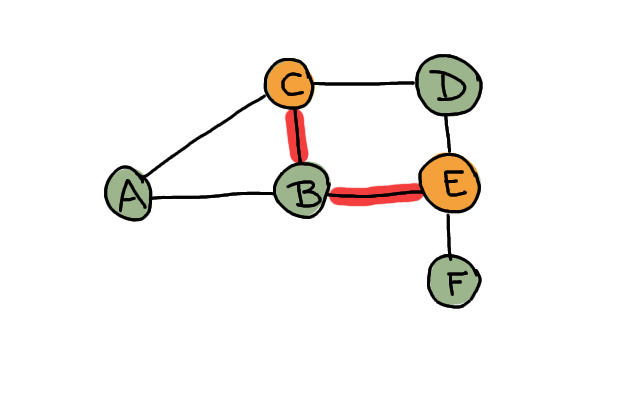
\includegraphics[width=0.5\textwidth]{Pictures/SP/abstand_ex-l2.png}
\end{figure}

\paragraph{Aufgabe \ref{aufgabe_abstand}}
\begin{enumerate}[(a)]
\item Der vollständige Graph mit 5 Knoten hat eine Kante zwischen jedem Paar von Knoten. Da jeder Knoten mit jedem anderen direkt verbunden ist, ist der Abstand zwischen zwei beliebigen Knoten \(1\).
\begin{figure}[H]
    \centering
    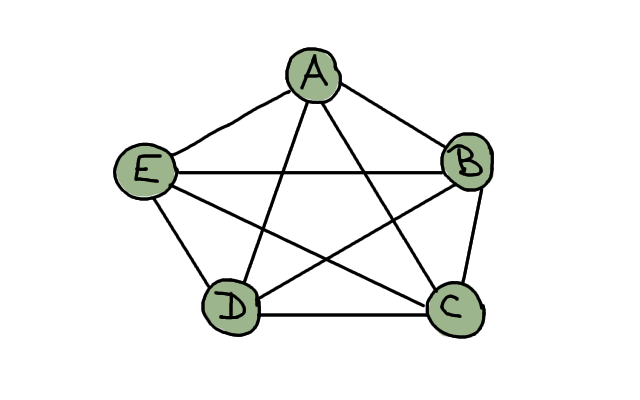
\includegraphics[width=0.5\textwidth]{Pictures/SP/abstand_k5.png}
\end{figure}

\item In einem 2 mal 3 Gittergraphen die Knoten sind in 2 Reihen und 3 Spalten organisiert und jeder Knoten ist mit den linken, rechten, oberen und unteren Nachbarn verbunden. Die zwei Knoten, die am weitesten auseinander liegen, sind die zwei diagonal zueinander stehende Ecken. Der Weg zwischen zwei solchen Ecken liegt durch die ganze Breite und die ganze Höhe des Gitters. In diesem Fall der maximale Abstand ist \(3\).
\begin{figure}[H]
    \centering
    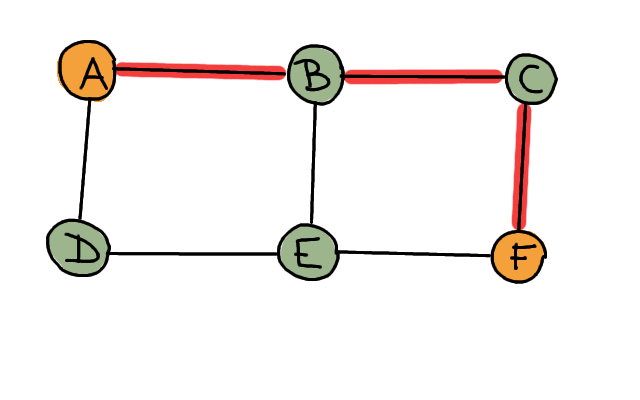
\includegraphics[width=0.5\textwidth]{Pictures/SP/abstand_gitter23.png}
\end{figure}

\item In einem Kreis gibt es zwei Pfade zwischen zwei beliebige Knoten. Zum Beispiel, zwischen \textbf{A} und \textbf{F} haben wir die Pfade \textbf{ABCDEF} und \textbf{AF}. Damit der kürzeste Pfad am Längsten wird, müssen diese zwei Pfade ungefähr gleich lang sein. Die zwei Knoten, die am weitesten ausenander sind, sind also gegenüberliegend.
\begin{figure}[H]
    \centering
    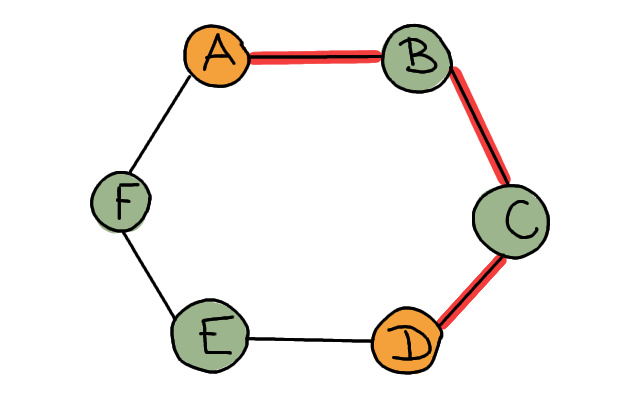
\includegraphics[width=0.5\textwidth]{Pictures/SP/abstand_kreis6.png}
\end{figure}
\end{enumerate}

\paragraph{Augabe \ref{aufgabe_panda_gebissen}}
\begin{enumerate}[(a)]
\item Die Knoten sind die genannten Leuten (Alice, Bob, Charlie, David, Elisabeth, Fred, Gregory, Hannah, Jakob, Lucy). Zwischen zwei Knoten gibt es eine Kante, wenn die entsprechenden Leuten sich irgendwoher schon kennen. Der Graph sieht dann so aus (wenn wir die Knoten mit dem ersten Buchstaben des Vornamens beschriften). Der Graph ist ungerichtet, weil wenn Person A Person B kennt, dann kennt Person B Person A auch.
    \begin{figure}[H]
        \centering
        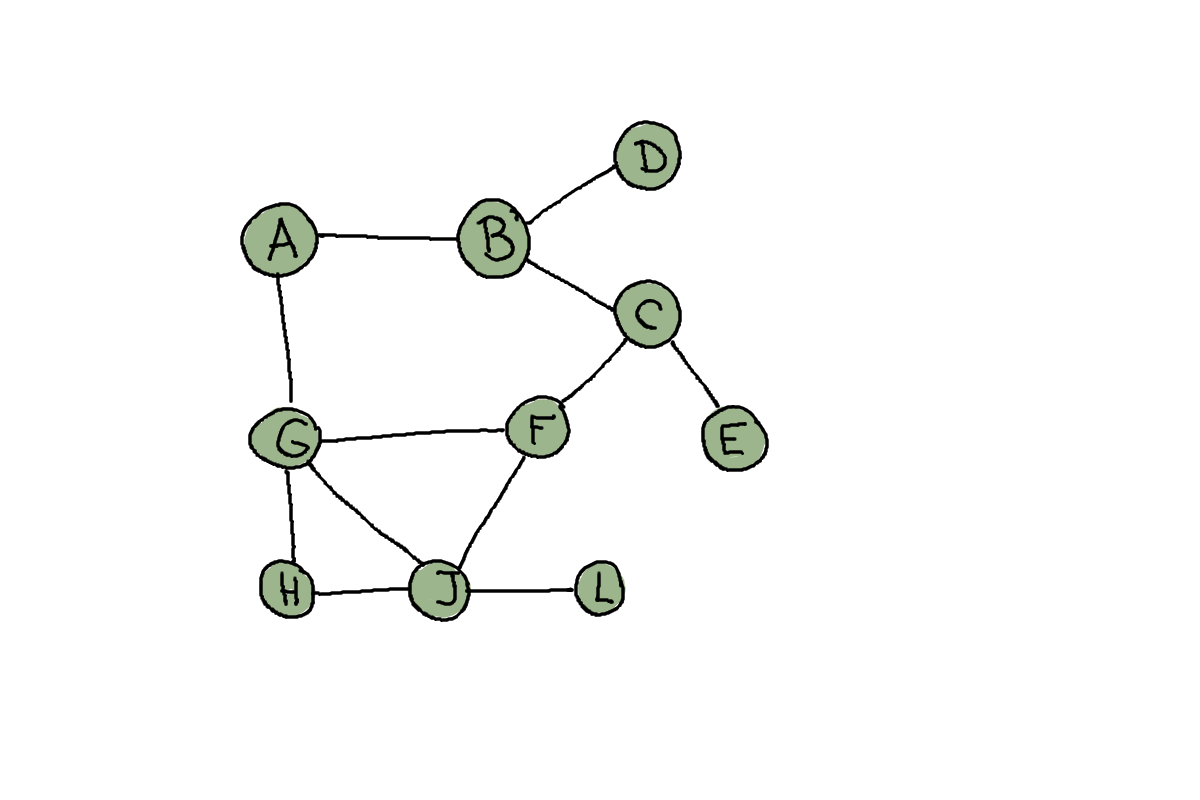
\includegraphics[width=\textwidth]{Pictures/SP/panda_gebissen_graph.png}
        \caption{Freundschaftsgraph}
        \label{fig:Gregory}
    \end{figure}

\item Wir markieren in grau die Knoten, die schon besucht worden sind und in Orange diejenigen, die sich in der Warteschlange befinden. In der Warteschlange schreiben wir unter dem Knoten auch den Abstand vom Startknoten auf.
\begin{figure}[H]
    \centering
    \begin{subfigure}[h]{0.45\textwidth}
    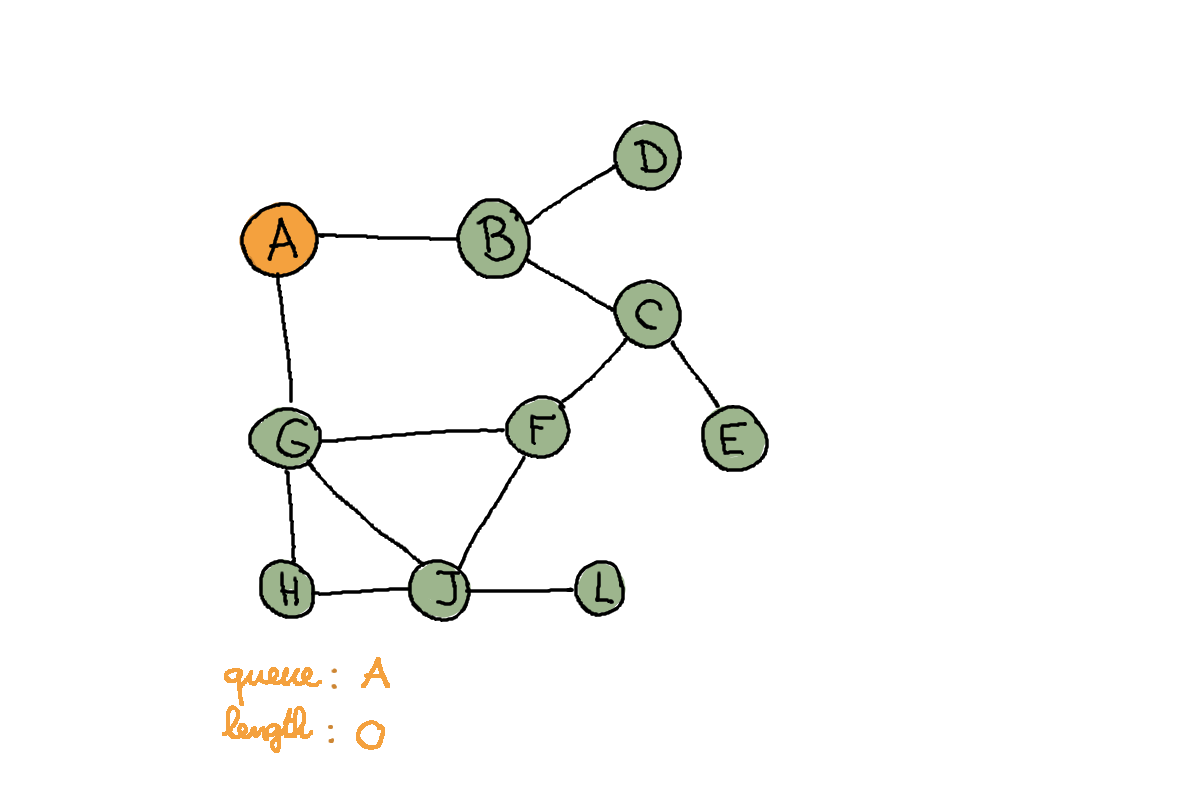
\includegraphics[width=\textwidth]{Pictures/SP/panda_gebissen_0.png}
    \end{subfigure}
    \vspace{5mm}
    \qquad
    \begin{subfigure}[h]{0.45\textwidth}
    \raggedleft
    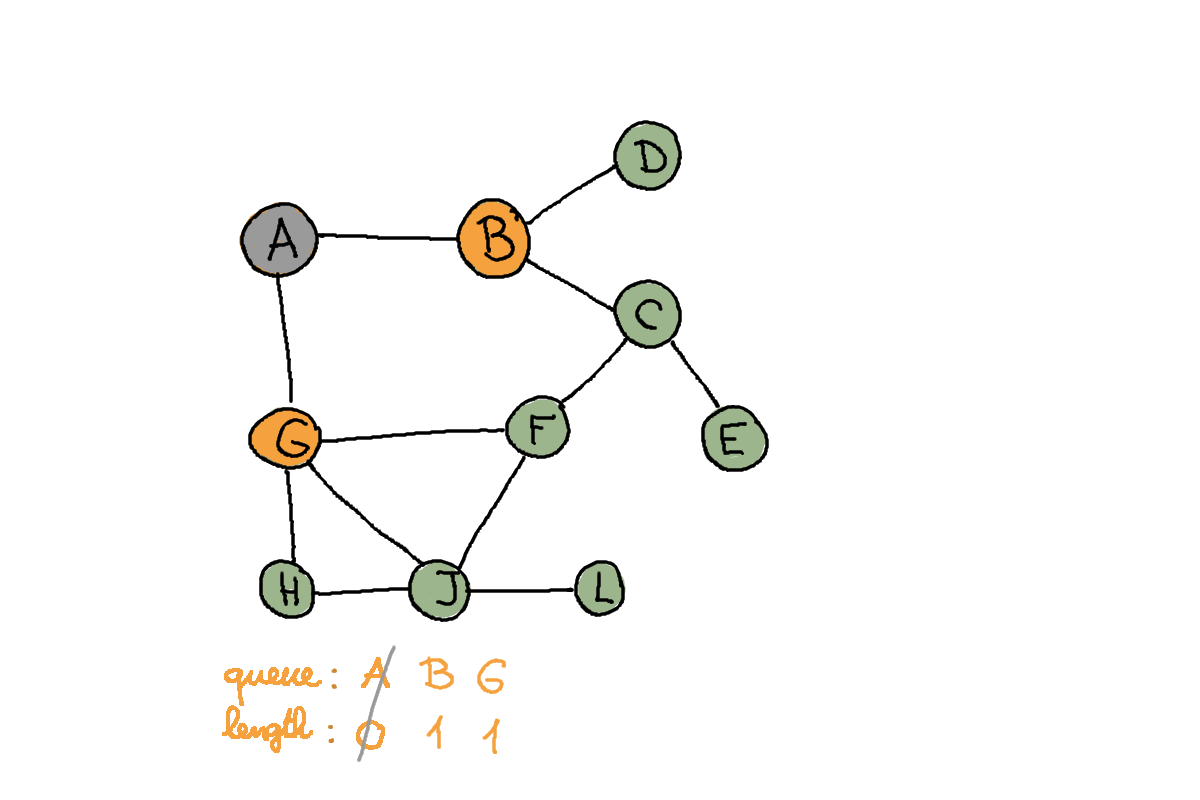
\includegraphics[width=\textwidth]{Pictures/SP/panda_gebissen_1.png}
    \end{subfigure}
    \vspace{5mm}
    \centering
    \begin{subfigure}[h]{0.45\textwidth}
    \raggedright
    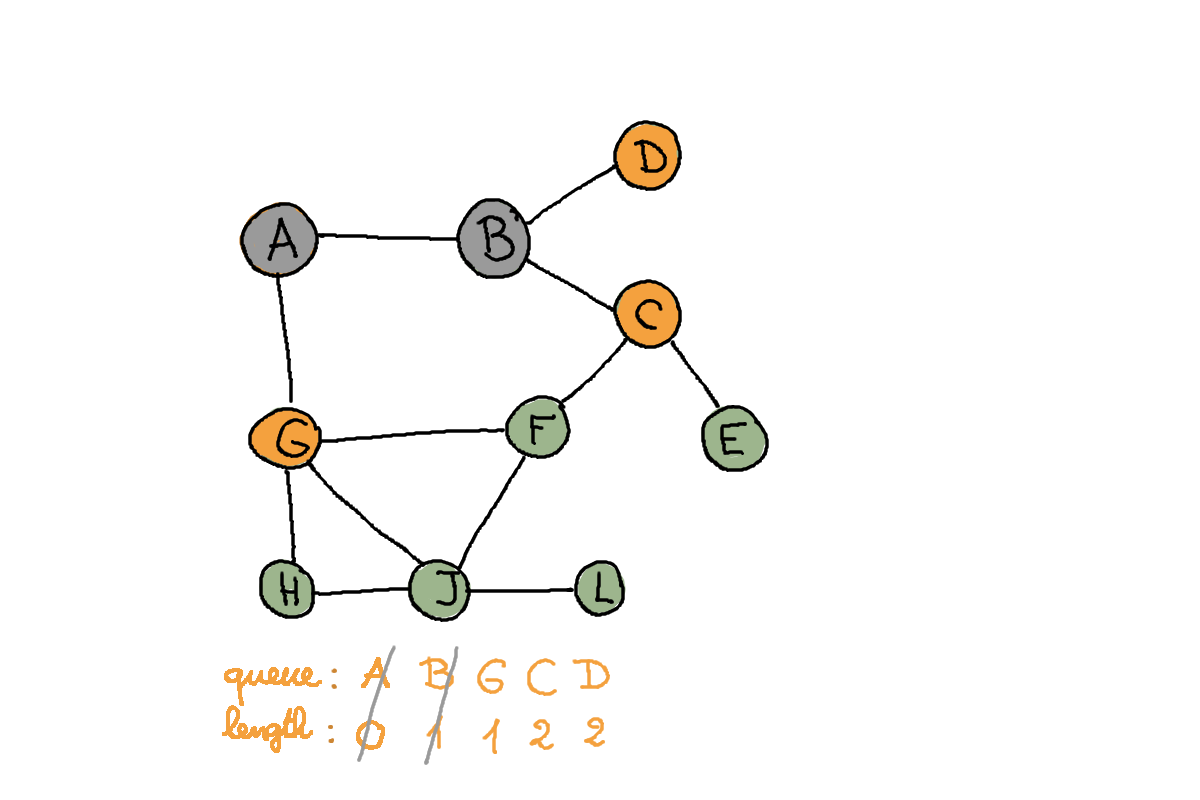
\includegraphics[width=\textwidth]{Pictures/SP/panda_gebissen_2.png}
    \end{subfigure}
    \qquad
    \begin{subfigure}[h]{0.45\textwidth}
    \raggedleft
    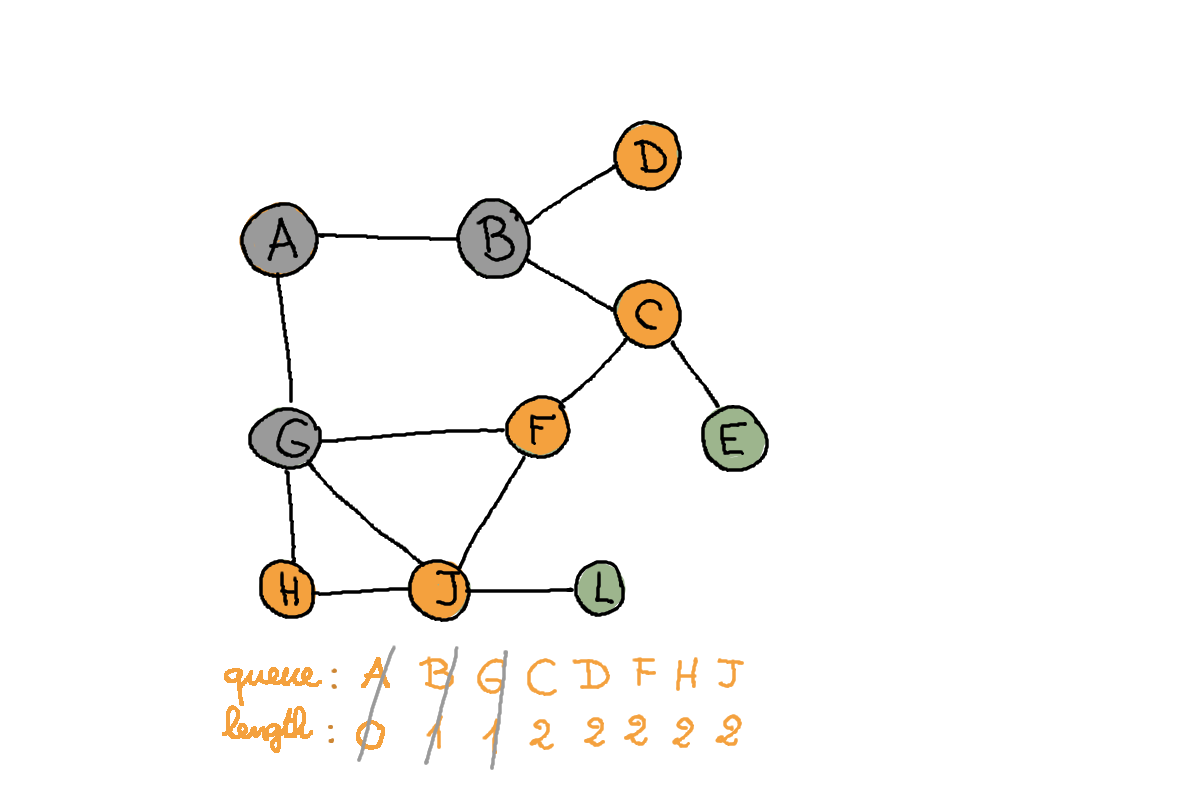
\includegraphics[width=\textwidth]{Pictures/SP/panda_gebissen_3.png}
    \end{subfigure}
\end{figure}
\begin{figure}[H]\ContinuedFloat
    \begin{subfigure}[h]{0.45\textwidth}
    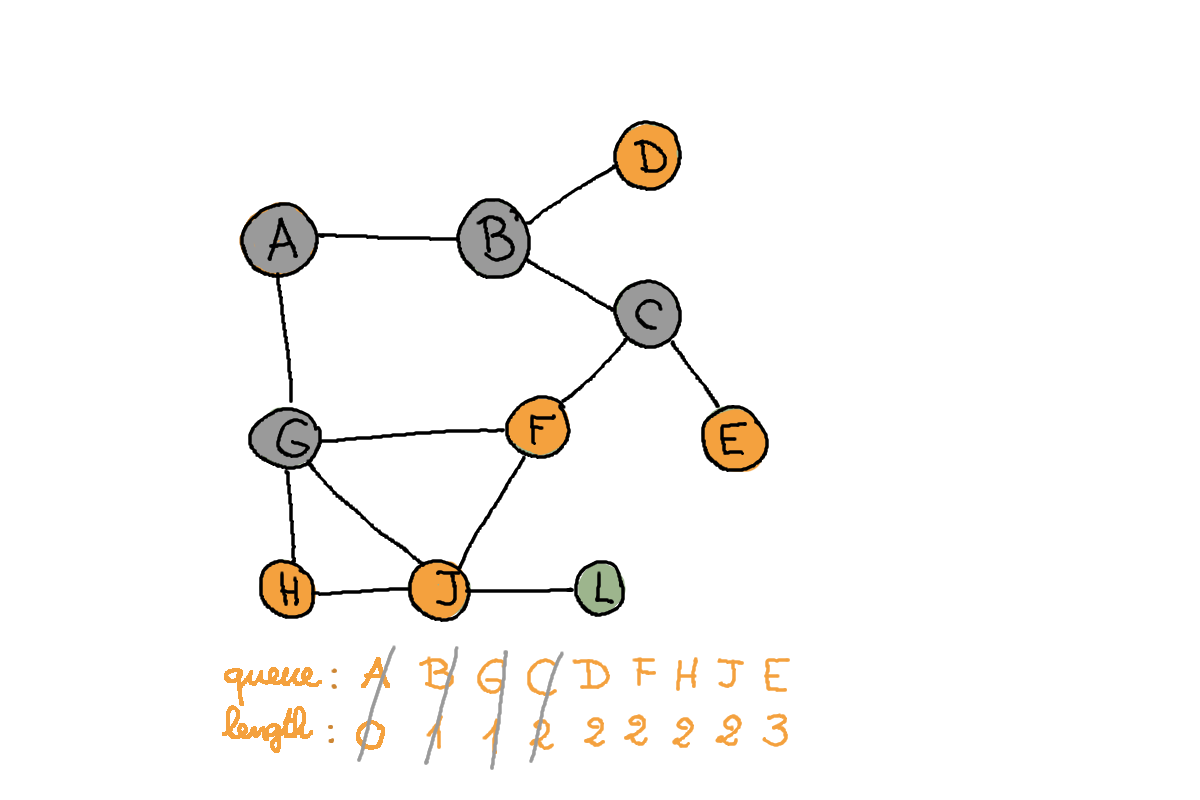
\includegraphics[width=\textwidth]{Pictures/SP/panda_gebissen_4.png}
    \end{subfigure}
    \vspace{5mm}
    \qquad
    \begin{subfigure}[h]{0.45\textwidth}
    \raggedleft
    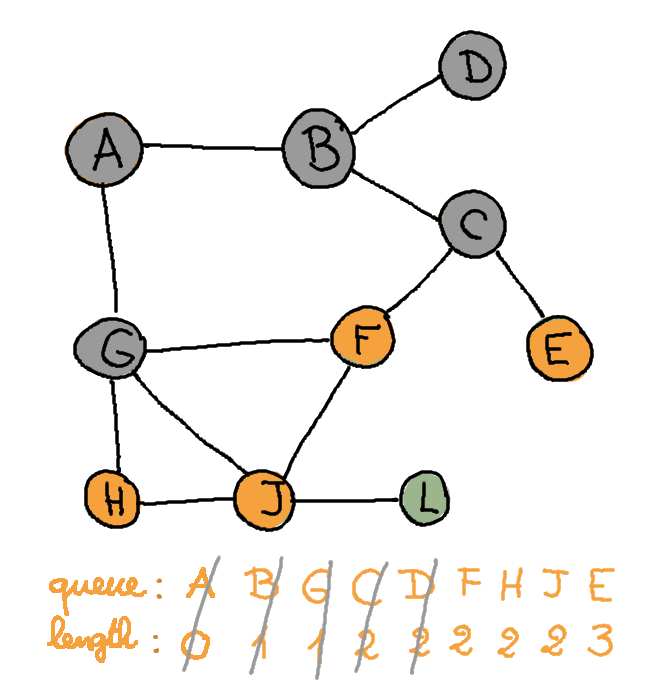
\includegraphics[width=\textwidth]{Pictures/SP/panda_gebissen_5.png}
    \end{subfigure}
    \vspace{5mm}
    \centering
    \begin{subfigure}[h]{0.45\textwidth}
    \raggedright
    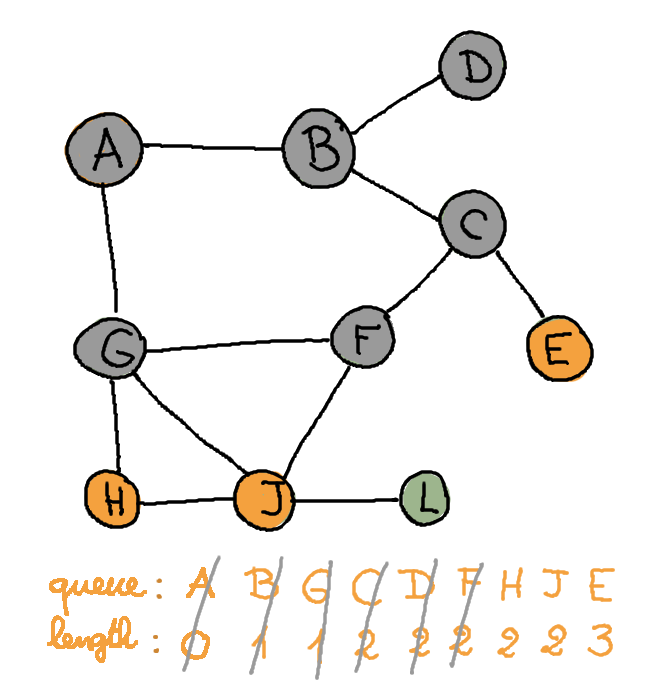
\includegraphics[width=\textwidth]{Pictures/SP/panda_gebissen_6.png}
    \end{subfigure}
    \qquad
    \begin{subfigure}[h]{0.45\textwidth}
    \raggedleft
    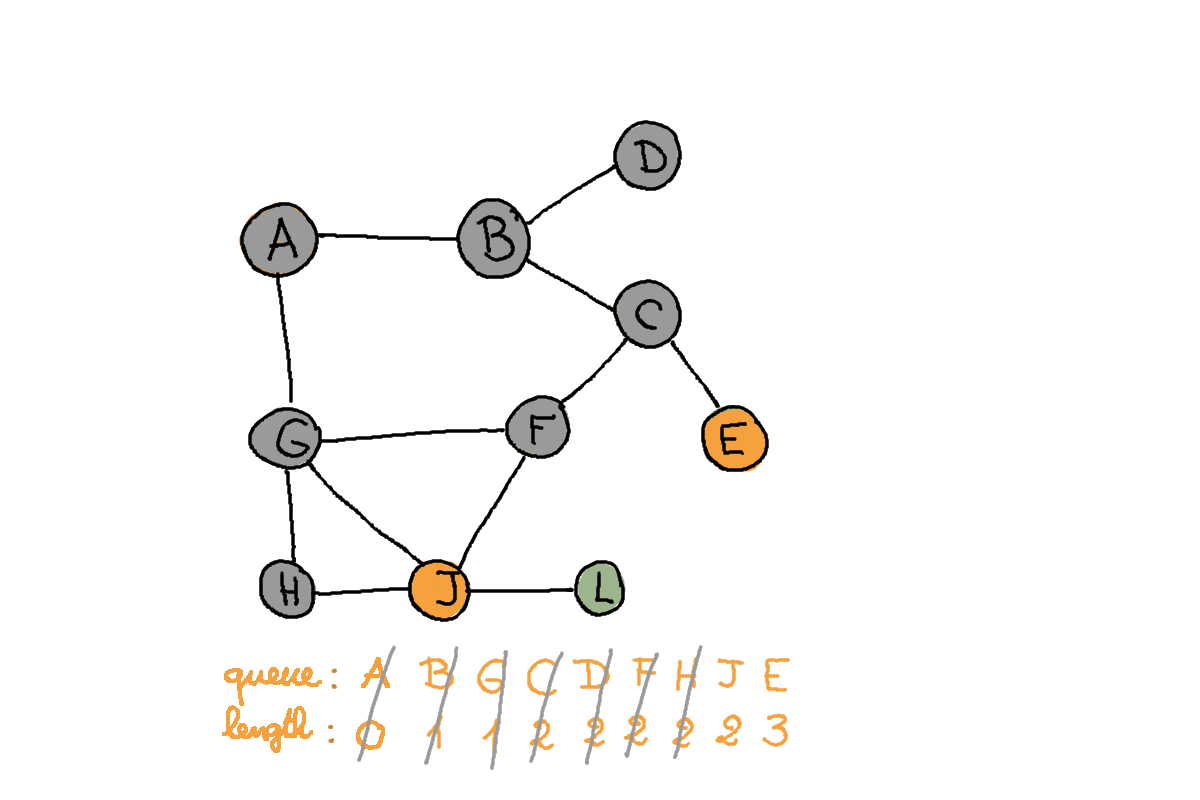
\includegraphics[width=\textwidth]{Pictures/SP/panda_gebissen_7.png}
    \end{subfigure}
\end{figure}
\begin{figure}[H]\ContinuedFloat
	\centering
    \begin{subfigure}[h]{0.6\textwidth}
    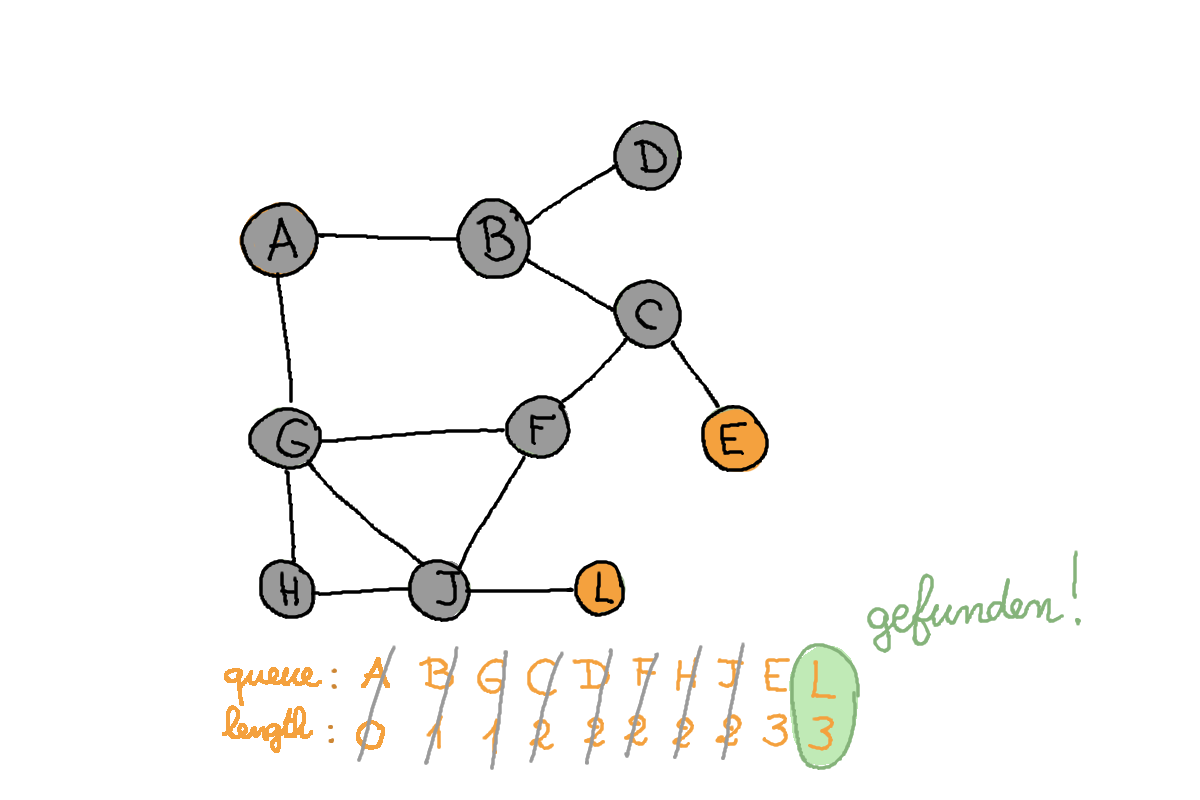
\includegraphics[width=\textwidth]{Pictures/SP/panda_gebissen_8.png}
    \end{subfigure}
\end{figure}
\item 
\begin{lstlisting}[language=Python, caption={Freundschaftsgraph in der Liste der Nachbarn Darstellung.}]
friends = {"A":["B", "G"],
        "B":["A", "C", "D"],
        "C":["B", "E", "F"],
        "D":["B"],
        "E":["C", "F"],
        "F":["C", "E", "G", "J"],
        "G":["A", "F", "H", "J"],
        "H":["G", "J"],
        "J":["F", "G", "H", "L"],
        "L":["J"]}
\end{lstlisting}
\item Dieser Graph ist klein und wir können durch Ausprobieren bestimmen, dass die zwei Knoten, die am weitesten auseinander sind, sind \textbf{D} und \textbf{L} und der Abstand zwischen diesen zwei Knoten ist \(5\).
\begin{lstlisting}[language=Python]
print(length_shortest_path(friends, "D", "L"))
5
\end{lstlisting}
Wir können aber auch ein Programm schreiben, das uns die Länge vom längsten kürzesten Pfad (den Diameter) ausrechnet. Dafür werden wir zunächst Programm \ref{lst:length_shortest_path} so umschreiben, dass es die Längen von allen kürzesten Pfaden vom Startknoten aus ausgibt. Die zwei grössten Änderungen sind, dass wir die Abstände nun auch in \texttt{visited} reinschreiben, so dass wir sie ausgeben können, und dass wir die Suche nicht mehr abbrechen, wenn wir den Endknoten gefunden haben (deswegen geben wir dem Programm auch keinen Endknoten mit).
\begin{lstlisting}[language=Python, caption={Programm, welches die Abstände vom Startknoten zu allen anderen erreichbaren Knoten ausrechnet}]
def length_all_shortest_paths_from(graph, initial):
    queue = [(initial, 0)]
    visited = {initial: 0}
    while queue:
        (node, length) = queue.pop(0)
        newlength = length + 1
        neighbours = graph[node]
        for neighbour in neighbours:
            if neighbour not in visited.keys():
                queue.append((neighbour, newlength))
                visited[neighbour] = newlength
    return visited
\end{lstlisting}
Jetzt können wir dieses Programm verwenden, um den Diameter auszurechnen. Wir gehen durch alle Knoten im Graphen durch und rufen \texttt{length\_all\_shortest\_paths\_from} auf. Das gibt uns für jeden Knoten die Abstände zu allen anderen erreichbaren Knoten im Graphen. Dann nehmen wir das Maximum über all diesen kürzesten Pfade und somit bestimmen wir den Diameter.
\begin{lstlisting}[language=Python, caption={Programm, welches den Diameter von einem Graphen bestimmt}]
def diameter(graph):
    maximum = (0, "from", "to")
    for node in graph.keys():
        all_shortest_from = length_all_shortest_paths_from(graph, node)
        farthest_from_node = max(all_shortest_from, key=all_shortest_from.get)
        if (all_shortest_from[farthest_from_node] > maximum[0]):
            maximum = (all_shortest_from[farthest_from_node], node, farthest_from_node)
    return maximum
\end{lstlisting}
Wenn wir dieses Programm ausführen, erfahren wir, dass der Diameter vom Fraundschaftsgraphen 5 ist, und dass der Abstand zwischen \texttt{D} und \texttt{L} genau diesen Wert hat.
\begin{lstlisting}[language=Python]
print(diameter(friends))
(5, 'D', 'L')
\end{lstlisting}
\end{enumerate}

\paragraph{Aufgabe \ref{aufgabe_shortest_path}}
Zuerst verwenden wir die Breitensuche, um alle Elternknoten zu ermitteln. Dann führen wir \texttt{backtracking} aus.
\begin{lstlisting}[language=Python]
def shortest_path(graph, initial, goal):
    parents = bfs_with_parent(graph, initial)
    return backtracking(parents, goal)
\end{lstlisting}

\paragraph{Aufgabe \ref{aufgabe_erde_mars_graph}}
\begin{enumerate}[(a)]
    \item Die Knoten sind die Wörter aus der Liste. Es gibt genau dann eine Kante zwischen zwei Wörter, wenn die Wörter sich um genau einen Buchstaben unterscheiden, wie zum Beispiel \texttt{MARS} und \texttt{MARK}. Der Graph ist ungerichtet, weil wenn sich ein Wort A um einen Buchstaben von einem Wort B unterscheidet, dann unterscheidet sich auch Wort B vom Wort A um einen Buchstaben.
    
    \item Der Graph sieht fol­gen­der­ma­ssen aus:
    \begin{figure}[H]
    \centering
    \includegraphics[width=0.6\textwidth]{Pictures/SP/bank_zins.png}
\end{figure}

	\item Ja, der Pfad ist
	\begin{lstlisting}
BANK - ZANK - ZINK - ZINS.
	\end{lstlisting}
	
	\item Ja, es reicht sogar ein Wort: \texttt{SIND}. Dann der Pfad wäre
	\begin{lstlisting}
BANK - SANK - SAND - SIND - SINN - ZINN - ZINS.
	\end{lstlisting}
	\begin{figure}[H]
    \centering
    \includegraphics[width=0.6\textwidth]{Pictures/SP/bank_zins_sind.png}
\end{figure}	
\end{enumerate}

\paragraph{Aufgabe \ref{aufgabe_erde_mars_neighbours}}
\begin{enumerate}[(a)]
    \item
    \begin{lstlisting}[language=Python]
words = {"ERDE":["EIDE", "ENDE", "ERLE"],
    "EIDE":["EILE", "EINE", "ENDE", "ERDE"],
    "EINE":["EIDE", "EILE", "EINS"],
    "EINS":["EINE", "PINS", "ZINS"],
    "ZINS":["EINS", "PINS", "ZINK", "ZINN"],
    "ZINK":["ZINS", "ZINN", "ZANK", "ZICK"],
    "ZANK":["BANK", "SANK", "ZACK", "ZINK"],
    "ZACK":["ZANK", "PACK", "ZICK", "SACK"],
    "PACK":["ZACK", "SACK", "PARK"],
    "PARK":["PACK", "PARD", "MARK"],
    "MARK":["PARK", "MARS"],
    "MARS":["MARK", "MAUS"],
    "MAUS":["MARS", "HAUS"],
    "HAUS":["MAUS", "HASS"],
    "HASS":["HAUS", "BASS"],
    "BASS":["HASS"],
    "PARD":["PARK"],
    "BAND":["SAND", "BANK"],
    "SAND":["BAND", "SANK"],
    "SACK":["SANK", "ZACK", "PACK"],
    "BANK":["BAND", "SANK", "ZANK"],
    "SANK":["BANK", "ZANK", "SACK", "SAND"],
    "SINN":["ZINN"],
    "ZINN":["SINN", "ZINK", "ZINS"],
    "ZICK":["ZINK", "ZACK"],
    "PINS":["ZINS","EINS"],
    "EILT":["EILE"],
    "EILE":["EINE", "EILT", "EULE"],
    "EULE":["EILE", "ERLE"],
    "ERLE":["EULE", "ERDE"],
    "ENDE":["ERDE", "EIDE", "ENTE"],
    "ENTE":["ENDE"]}
    \end{lstlisting}
    
    \item
    \begin{lstlisting}[language=Python]
print(shortest_path(words, "ERDE", "MARS"))
['ERDE', 'EIDE', 'EINE', 'EINS', 'ZINS', 'ZINK', 'ZANK', 'ZACK', 'PACK', 'PARK', 'MARK', 'MARS']
    \end{lstlisting}
    
    \item Die Idee ist, dass wir zuerst für den ersten Buchstaben alle 26 Möglichkeiten ausprobieren. Wenn wir auf dieser Art und Weise ein Wort aus der Referenzliste kriegen, dann fügen wir es zu den Nachbarn hinzu. Mit dem zweiten, dritten und vierten Buchstaben gehen wir analog vor.
    \begin{lstlisting}[language=Python]
def compute_neighbours(nodes, node):
    neighbours = []
    for c1 in string.ascii_uppercase:
        neighbour = c1+node[1:4]
        if neighbour != node:
            if neighbour in nodes:
                neighbours.append(neighbour)
                
    for c2 in string.ascii_uppercase:
        neighbour = node[0]+c2+node[2:4]
        if neighbour != node:
            if neighbour in nodes:
                neighbours.append(neighbour)
    
    for c3 in string.ascii_uppercase:
        neighbour = node[0:2]+c3+node[3:4]
        if neighbour != node:
            if neighbour in nodes:
                neighbours.append(neighbour)
                
    for c4 in string.ascii_uppercase:
        neighbour = node[0:3]+c4
        if neighbour != node:
            if neighbour in nodes:
                neighbours.append(neighbour)
    return neighbours
    \end{lstlisting}
    Dieses Programm kann eleganter gemacht werden, indem man eine Schleife anstatt von den vier ähnlichen Blöcke verwendet.
    
    \item Das Programm, welches den kürzesten Pfad berechnet, ruft zwei Programme auf: \texttt{bfs\_with\_parent} und \texttt{backtracking}. In \texttt{bfs\_with\_parent} haben wir die nicht besuchten Nachbarn aus dem Graphen in der Liste der Nachbarn Darstellung einfach ablesen können. Nun werden wir aber nur die Liste aller Knoten (auch Referenzliste in der vorherigen Teilaufgabe genannt) herumreichen. Die Nachbarn eines Knotens müssen wir also mit \texttt{compute\_neighbours} (siehe vorherige Teilaufgabe) berechnen. Das \texttt{backtracking} Programm bleibt hingegen unverändert.
    \begin{lstlisting}[language=Python]
def bfs_with_parent_neighbours(nodes, initial):
    queue = [initial]
    visited = {initial:None}
    while queue:
        node = queue.pop(0)
        neighbours = compute_neighbours(nodes, node)
        for neighbour in neighbours:
            if neighbour not in visited:
                queue.append(neighbour)
                visited[neighbour] = node
    return visited
    
def shortest_path_neighbours(nodes, initial, goal):
    parents = bfs_with_parent_neighbours(nodes, initial)
    return backtracking(parents, goal)
    \end{lstlisting}  
\end{enumerate}

\paragraph{Aufgabe \ref{aufgabe_schlangenspiel}}
\begin{enumerate}[(a)]
    \item Die Knoten sind die Kästchen, wo die Zahlen stehen. Zwischen Knoten A und Knoten B gibt es eine Kante, wenn Kästchen B aus dem Kästchen A mit einem Würfelwurf erreicht werden kann (inklusive Schlagen- und Leiterzauber). Der Graph ist gerichtet, weil man nicht zurück oder in der Gegenrichtung von Zauberkästchen gehen kann.
    \item Eine mögliche Darstellung ist:
    \begin{lstlisting}[language=Python]
snakes_and_ladders = {
    0: [1, 3, 5, 11],
    1: [3, 5, 11],
    2: [3, 5, 6, 11],
    3: [1, 5, 6, 11],
    4: [1, 5, 6, 8],
    5: [1, 6, 8, 9],
    6: [1, 3, 8, 9],
    7: [3, 8, 9, 11],
    8: [3, 9, 11],
    9: [3, 11],
    10: [11],
    11: []
}
    \end{lstlisting}
    
    \item
    \begin{lstlisting}[language=Python]
print(shortest_path(snakes_and_ladders, 0, 11))
[0, 11]
    \end{lstlisting}
    Bob muss eine 4 Würfeln, dann hat er beim ersten Wurf gewonnen.
    
    \item Wir können die Liste der Nachbarn so umschreiben, dass wir die gewürfelte Zahl mitgeben. Dann können wir diese Zahl als Teil vom Nachbarn herumreichen.
    \item Wir brauchen zusätzlich ein Wörterbuch, welches die Zauberfelder (Schlangen und Leiter) auf die effektiven Felder übersetzt. Auf dem kleinen Spielfeld würde das Wörterbuch so aussehen.
    \begin{lstlisting}[language=Python]
magic_squares = {
    2: 5,
    4: 11,
    7: 1,
    10: 3
}
    \end{lstlisting}
    Um die Nachbarn zu ermitteln, addieren wir die gewürfelte Zahl und dann übersetzen wir sie mit dem Wörterbuch, um ''Zauberfelber'' richtig zu behandeln.
    
    Wir müssen jetzt bestimmen, was passiert, wenn man eine zu hohe Zahl würfelt. Das einfachste ist den Spieler in einem solchen Fall gewinnen zu lassen. Dafür mussen wir noch ein paar ''Zauberfelder'' einfügen.
    \begin{lstlisting}[language=Python]
magic_squares = {
    2: 5,
    4: 11,
    7: 1,
    10: 3,
    12: 11,
    13: 11,
    14: 11,
    15: 11
}
    \end{lstlisting}
    Dieses Programm gibt manche Nachbarn doppelt aus, aber bei der Breitensuche, wo wir den \texttt{visited}-Vektor haben, wird es keinen Effekt auf die Korrektheit haben.
    \begin{lstlisting}[language=Python]
def compute_neighbours(magic_dict, node):
    neighbours = []
    for i in [1, 2, 3, 4]:
        neighbour = node + i
        if neighbour in magic_dict.keys():
            neighbour = magic_dict[neighbour]
        neighbours.append(neighbour)
    return neighbours
    \end{lstlisting}{}
    
    \item Zuerst modifizieren wir \texttt{compute\_neighbours} so, dass wir nicht nur die Nachbarn berechnen sondern auch die gewürfelten Zahlen nicht verlieren.
    \begin{lstlisting}[language=Python]
def compute_neighbours_and_dice(magic_dict, node):
    neighbours = []
    for i in [1, 2, 3, 4]:
        neighbour = node + i
        if neighbour in magic_dict.keys():
            neighbour = magic_dict[neighbour]
        neighbours.append((neighbour, i))
    return neighbours
    \end{lstlisting}
    
    Dann schreiben wir \texttt{bfs\_with\_parent} um, so dass wir die gewürfelten Zahlen nicht verlieren.
    \begin{lstlisting}
def bfs_with_parent_and_dice(magic_dict, initial):
    queue = [initial]
    visited = {initial:(None, None)}
    while queue:
        node = queue.pop(0)
        neighbours_and_die = compute_neighbours_and_dice(magic_dict, node)
        for (neighbour, dice) in neighbours_and_die:
            if neighbour not in visited:
                queue.append(neighbour)
                visited[neighbour] = (node, dice)
    return visited
    \end{lstlisting}
    
    Dieses Mal müssen wir das \texttt{backtracking} Programm umschreiben, weil wir anstatt von den Knoten die gewürfelten Zahlen ausgeben wollen.
    \begin{lstlisting}[language=Python]
def backtracking_dice(parents_and_dice, goal):
    reversed_path = []
    (node, dice) = parents_and_dice[goal]
    while node != None:
        reversed_path.append(dice)
        (node, dice) = parents_and_dice[node]
    return list(reversed(reversed_path))
    \end{lstlisting}
    
    Jetzt können wir wie gewohnt alle Teile zusammensetzen.
    \begin{lstlisting}[language=Python]
def shortest_path_neighbours_and_dice(magic_dict, initial, goal):
    parents_and_dice = bfs_with_parent_and_dice(magic_dict, initial)
    return backtracking_dice(parents_and_dice, goal)
    \end{lstlisting}
    
    Wir sind endlich bereit, das grosse Schlangenspiel zu lösen.
    \begin{lstlisting}[language=Python]
magic_squares_big = {
    39: 2,
    15: 5,
    17: 22,
    14: 35,
    56: 36,
    42: 55,
    26: 45,
    32: 13,
    9: 11,
    51: 30,
    60: 59,
    61: 59,
    62: 59,
    63: 59,
}

print(shortest_path_neighbours_and_dice(magic_squares_big, 0, 59))
[1, 4, 4, 3, 3, 4, 4]
    \end{lstlisting}
    Es ist möglich, das grosse Schlangenspiel in 7 Würfe zu gewinnen, wenn man jedes Mal die richtige Zahl würfelt.
\end{enumerate}













\end{document}
